In Chapter \ref{ch:usbe_lung} we introduced the problem of
\ac{DUS}-induced lung hemorrhage, however, the focus was on the
fundamental physical problem of an acoustically driven gas-liquid
interface, such as those of the alveoli. In this chapter, we aim to
extend that work to increase its relevance to \ac{DUS} of the
lung. Here, we hypothesize that real \ac{DUS} waves may be capable of
generating sufficient baroclinic vorticity at alveolar interfaces in
the lung to drive deformation and hemorrhage. To investigate this
hypothesis we again model the alveolus as a perturbed water-air
interface and examine the dynamics when driven by ultrasound pulses
with clinically relevant parameters. We compare the interface
evolution to that expected of a vorticity driven interface based on
the work of Chapter \ref{ch:usbe_lung}. Furthermore, we infer the
viscous stress and calculate the approximate strain at the interface
and compare computed values to expected alveolar damage thresholds,
based on previous published research.

\section{Abstract}
\ac{DUS}-induced lung hemorrhage in mammals is the only known
biological effect of non-contrast diagnostic ultrasound. Despite years
of study, the underlying physical mechanism remains unknown. In this
work we model the interaction between an ultrasound pulse and an
alveolus as an acoustic wave in water propagating toward a water-air
interface. To capture the alveolar surface roughness the interface
contains a single-mode sinusoidal perturbation, representing the
alveolar surface roughness, of variable initial amplitudes equal to 3,
10, and 30\% of the perturbation wavelength, which represents the
alveolar diameter. By solving the Euler equations of fluid motion we
study the evolution of the interface for 1.5 MHz ultrasound with peak
amplitudes of 1.0, 2.5, and 5.0 MPa. The interface is observed to
continue deforming long after the passage of the wave. Interfacial
strains of up to 38\% after 288 $\mu$s. Viscous stresses are estimated
and maximum amplitudes are found to be on the order of $10$ Pa. For a
10 MPa pulse, interface perturbation amplitudes are shown to grow
approximately as $t^{3/5}$, which is expected of vorticity-driven
growth based on the work of Chapter \ref{ch:usbe_lung}.

\section{Introduction}
Lung \ac{US} has become a common tool for imaging and diagnostics in
critical and point-of-care situations and its use is growing
\citep{Lichtenstein2009}. Currently, \ac{PCH} is the only biological
effect known to occur in mammals as a result of non-contrast
diagnostic ultrasound. It has been shown to occur under clinically
acceptable parameters with \ac{MI}$\leq1.9$ \citep{FDA1997} and peak
pressures as low as $1.0$ MPa \citep{Dalecki1997}. The physical
mechanism underlying this damage is still not well understood. While
the occurrence of hemorrhage as a result of diagnostic lung \ac{US}
has not been directly studied in human lungs for obvious ethical
reasons, an understanding of the underlying cause is important for the
development of evidence-based safety guidelines and regulations.

\ac{US}-induced \ac{LH} is not a new problem. It was first discovered
in mice over twenty years ago \citep{Child1990}. And since then, there
has been considerable work to progress our understanding. Much of this
previous research has primarily aimed at three specific ends: (1)
investigating the physical damage mechanism causing the hemorrhage;
(2) determining the dependence of damage characteristics and
bioeffects thresholds on the \ac{US} properties; and (3) determining
the dependence of damage characteristics and thresholds on the
characteristics of the \ac{US} subject. This study aims to contribute
to the first of these areas: we aim to estimate the potential stresses
and strains imparted by a single ultrasound pulse on a perturbed
liquid-gas interface, similar to that of a single alveolus. To do this
we will extend the computational fluids model of an \ac{US}-driven
alveolus developed in Chapter \ref{ch:usbe_lung} to include \ac{US}
pulse-like waveforms and interface geometries with larger perturbation
amplitudes than previously considered, which are more representative
of physical alveoli.

In Chapters \ref{ch:Introduction} and \ref{ch:usbe_lung}, a portion of
the body of past research into the physical mechanisms of \ac{DUS} was
reviewed, so only a brief summary is provided
here. \ac{US}-induced pulmonary hemorrhage is characterized by alveoli
filling with blood as well as plasma proteins and erythrocytes
\citep{Miller2016a,Penney1993a}. Alveolar edema or frank hemorrhage
has also been shown to occur as a result of mechanical stress failure
of the alveolar membrane induced by over pressure
\citep{West1991}. The cause of \ac{DUS}-induced hemorrhage in the
lungs appears mechanical in nature and thermal mechanisms appear
unlikely to cause the observed damage \citep{Zachary2006,
  Dalecki2004}. Cavitation, acoustic radiation force, resonance, and
acoustic fountaining or atomization have all been studied as possible
mechanical damage mechanisms for \ac{DUS}-induced \ac{LH}
\citep{Holland1996,Miller2016a,Jabaraj2012,Jabaraj2013,Jabaraj2013a,Tjan2007,Simon2012}.
Experimental results suggest that the most common mechanical
ultrasound bioeffect mechanism, cavitation, is unlikely, and for
reasons detailed in the previous chapters, none of the remaining
mechanisms completely explains the damage \citep{OBrien2000,
  Raeman1996, Miller2016a}.

Research investigating the dependence of \ac{US}-induced \ac{LH} on
the characteristics of the \ac{US} subject has considered species,
age, physiological development, and pulmonary state of the \ac{US}
subject.  Within mammals, the occurrence of \ac{DUS}-induced \ac{LH}
has been observed to be largely species-indiscriminate and has been
found to occur in mice, pigs, rats, rabbits, and monkeys
\citep{Baggs1996, Child1990, Dalecki1997, Frizzell1994, Frizzell2003,
  Harrison1995, Holland1996, Kramer2001, OBrien1997a, OBrien2001b,
  OBrien2003a, OBrien2005, OBrien2000, OBrien2001a, Penney1993a,
  Raeman1993, Raeman1996, Tarantal1994a, Zachary1995a, Zachary2001a,
  Zachary2001}. \cite{Dalecki1997} subjected neonatal, juvenile, and
adult mice to pulsed ultrasound of the lung and observed that while
hemorrhage thresholds were similar in all mice, the degree of
hemorrhage was much greater in the adult mice than in the younger
subjects. Similarly, \cite{OBrien2003a}, studied the age dependence of
hemorrhage in pigs, and found that older pigs had a significantly
lower hemorrhage thresholds than juvenile and middle-aged pigs. In an
unexpected result, the study also found that if one lung was exposed
to \ac{US} and the pig was then rolled over and the second lung
exposed, the hemorrhage threshold in the second lung was substantially
lower than in the first. To study the dependence of hemorrhage on the
impedance boundary condition at the lung’s pleural surface,
\cite{OBrien2002a} subjected rats with variable degrees of lung
inflation to 3.1 MHz pulsed \ac{US} with \ac{PRPA} $=8.6, ~16$ MPa. It was
found that deflated lungs, which had less impedance mismatch with
their surroundings, were more easily damaged than partially deflated
lungs, which were more easily damaged than inflated lungs. While no
direct experimentation has been performed on humans, for obvious
ethical reasons, \cite{Meltzer1998} found that transesophageal
echocardiography with similar \ac{US} parameters to those causing lung
hemorrhage in animal studies ($3.1$ MHz, \ac{PRPA}$= 2.4$ MPa) did not
lead to visible hemorrhage on the surface of the lung. While
\ac{DUS}-induced \ac{LH} has not been shown to occur in humans, its
occurrence in a wide variety of mammals under diagnostically relevant
conditions suggests a need for further investigation.

The body of research investigating the dependence of lung hemorrhage
on \ac{US} properties is extensive and has investigated the dependence
of hemorrhage occurrence and severity on a wide variety \ac{US}
parameters. \cite{Zachary1995a} used continuous-wave and pulsed-wave
\ac{US} in mice, rabbits, and pigs, and found that continuous- and
pulsed-wave-induced lesions appear macroscopically similar, but
differed microscopically. Hemorrhage induced by continuous wave
\ac{US} consisted primarily of plasma and contained some cells,
whereas pulsed-wave induced hemorrhage was composed mostly of cells
and contained little plasma. \cite{Raeman1996} subjected mice to 2.3
MHz pulsed \ac{US} with peak pressures up to 3 MPa and varying
exposure time and found that while threshold amplitudes appeared
insensitive to exposure time, suprathreshold damage increased with
increasing exposure. In a review of previous work, \cite{Miller2016a}
indicated that previously observed differences in bioeffects
thresholds between studies may be attributable to exposure duration
differences. \cite{OBrien2001} investigated the effects of \ac{US}
beamwidth and found that for rats subjected to 2.8 and 5.6 MHz
ultrasound, incidence, surface area, and volume of hemorrhage
increased with increasing beamwidth. It was noted that lung hemorrhage
is perhaps the only known beamwidth-dependent mechanical bioeffect of
\ac{US}. \cite{OBrien2003c} found evidence that increasing \ac{US}
pulse duration decreases the \acp{PRPA} threshold associated with a
5\% likelihood of lung hemorrhage in rats subjected to 2.8 MHz
ultrasound with peak amplitudes ranging from 4-9 MPa. Given that the
dependencies of bioeffects on waveform amplitude and frequency are not
fully understood, we consider the dependence of the alveolar wall
dynamics on acoustic wave amplitude.

Separately, the structure, mechanical behavior, and failure properties
of alveoli have been studied extensively and are of particular
interest to the present work. The alveoli can be thought of as a
network of openly connected, air-filled saccules with distinctly
irregular surfaces. Past research suggests that alveolar size is
species dependent \citep{Faffe2002}. While alveoli are not perfect
spheres, their mean diameters range from tens to hundreds of microns,
with reported values of 45 $\mu$m in mice and 200 $\mu$m in adult
humans \citep{Knust2008,Ochs2004}. The septa separating adjacent
alveoli are nearly planar structures that contain several tissue
layers and are coated with a thin layer of liquid surfactant
\citep{Gil1979,Reifenrath1975,Perlman2014}. Within the alveolar septa
surrounding the alveoli, are the pulmonary capillaries, a sheet-like
web which is almost completely unsupported by surrounding tissue
\citep{West1991}. Separating the blood from the air is a multi-layer
wall of tissues, $0.2$ - $0.3\mu$m thick, referred to as the blood-gas
or blood-air barrier \citep{West2000}. \cite{West1991} raised the
pulmonary capillary pressure of anesthetized rabbits and observed
consistent stress failure of the capillary and alveolar epithelium for
transmural at or above $40$ mmHg ($5.3$ kPa). It was observed that
failure corresponded to approximately $25$ mN/m wall tension in the
capillaries, and noted that ``this tension is small, comparable with
the tension in the alveolar wall associated with elastic recoil.''
The capillary wall stress at failure was calculated to be
approximately $8$ kPa. Alveolar wall strain has also been studied and
linear, alveolar strain due to normal tidal breathing is reported to
range from $0$ -- $5$\% for humans \citep{Roan2011}. \cite{Belete2010}
found that when subjected to cyclical linear stretch at 0.5 Hz for 30
minutes, rat alveolar epithelial cells experiencing linear strains of
$8\%$ or greater were frequently damaged, whereas those experiencing
strains of $3$ -- $6\%$ were often undamaged.

This work is the first to use a fully nonlinear, Euler-based
computational fluids approach to study the dynamics of an alveolus
driven by a single ultrasound pulse. Extending the alveolar model of
Chapter \ref{ch:usbe_lung}, we perform numerical experiments to
simulate the dynamics of gas-liquid interfaces driven by ultrasound
pulse waveforms within the clinically relevant range. Using simple
models, we approximate the linear interfacial strain and infer viscous
stress at the interface, which we compare to alveolar failure criteria
from relevant literature. Additionally, we compare the interface
evolution to that expected of a vorticity-driven growth of interfacial
perturbation, based on our past work \citep{Patterson2017,Patterson2017b}.

%%%%%%%%%%%%%%%%%%%%%%%%%%%%%%% 
\section{Methods}
Much of the basic problem setup and computational framework detailed
in Chapter \ref{ch:usbe_lung} are reused here. In this section we
briefly summarize the model and then focus specifically on three
specific areas where changes have been to better suit our focus on
\ac{DUS}-induced \ac{LH}: (1) problem geometry, (2) incoming waveform,
(3) calculation of stress and strain.

v% \subsection{Summary of the model problem}
% We consider the problem of a single outermost alveolus driven by a
% single \ac{DUS} pulse, initially trAveling In adjacent to soft
% tissue. We model this problem as an \ac{US} wave in water impinging
% upon a sinusoidally perturbed air interface. This is consistent with
% the idea of alveoli as a network of openly connected, air-filled
% saccules with distinctly irregular surfaces. As such they have no true
% ``diameter'', but as past research suggests that their size appear to
% be species dependent \citep{Faffe2002}, we restrict our model and
% consider only an adult human alveolus which has a characteristic mean
% diameter of 200 $\mu$m \citep{Ochs2004}.

In the previous chapter, we simulated trapezoidal acoustic waves
impinging upon a nearly planar interface with a sinusoidal
perturbation. The width of the domain represents a single alveolar
diameter, $\ell=200 \mu$m in adult humans \citep{Ochs2004}, which is
also the wavelength of the perturbation. The initial perturbation
amplitude used $a_0=0.03\ell$, implies a nearly flat alveolar surface,
which is not always the case, as can be seen in the histological cross
section of alveoli shown in Figure \ref{fig:alveolar_histology}. To
account for the variety of geometries in alveolar tissue, many of
which are not particularly flat. A typical surface radius of curvature
for a human alveolus has been reported as $109~\mu$m
\citep{Mercer1994}. We will now consider perturbation amplitudes of
$a_0=0.03\ell, 0.10\ell$ and $a_0=0.30\ell$. We acknowledge that this
does not capture the true range of cross-sectional alveolar
geometries. However, this simplified geometry, necessitated by
computational constraints, will allow for the generalization of the
conclusions of this work broadly to relevant geometries.
\begin{figure}%
  \begin{subfigure}{0.45\textwidth}
    \centering%
    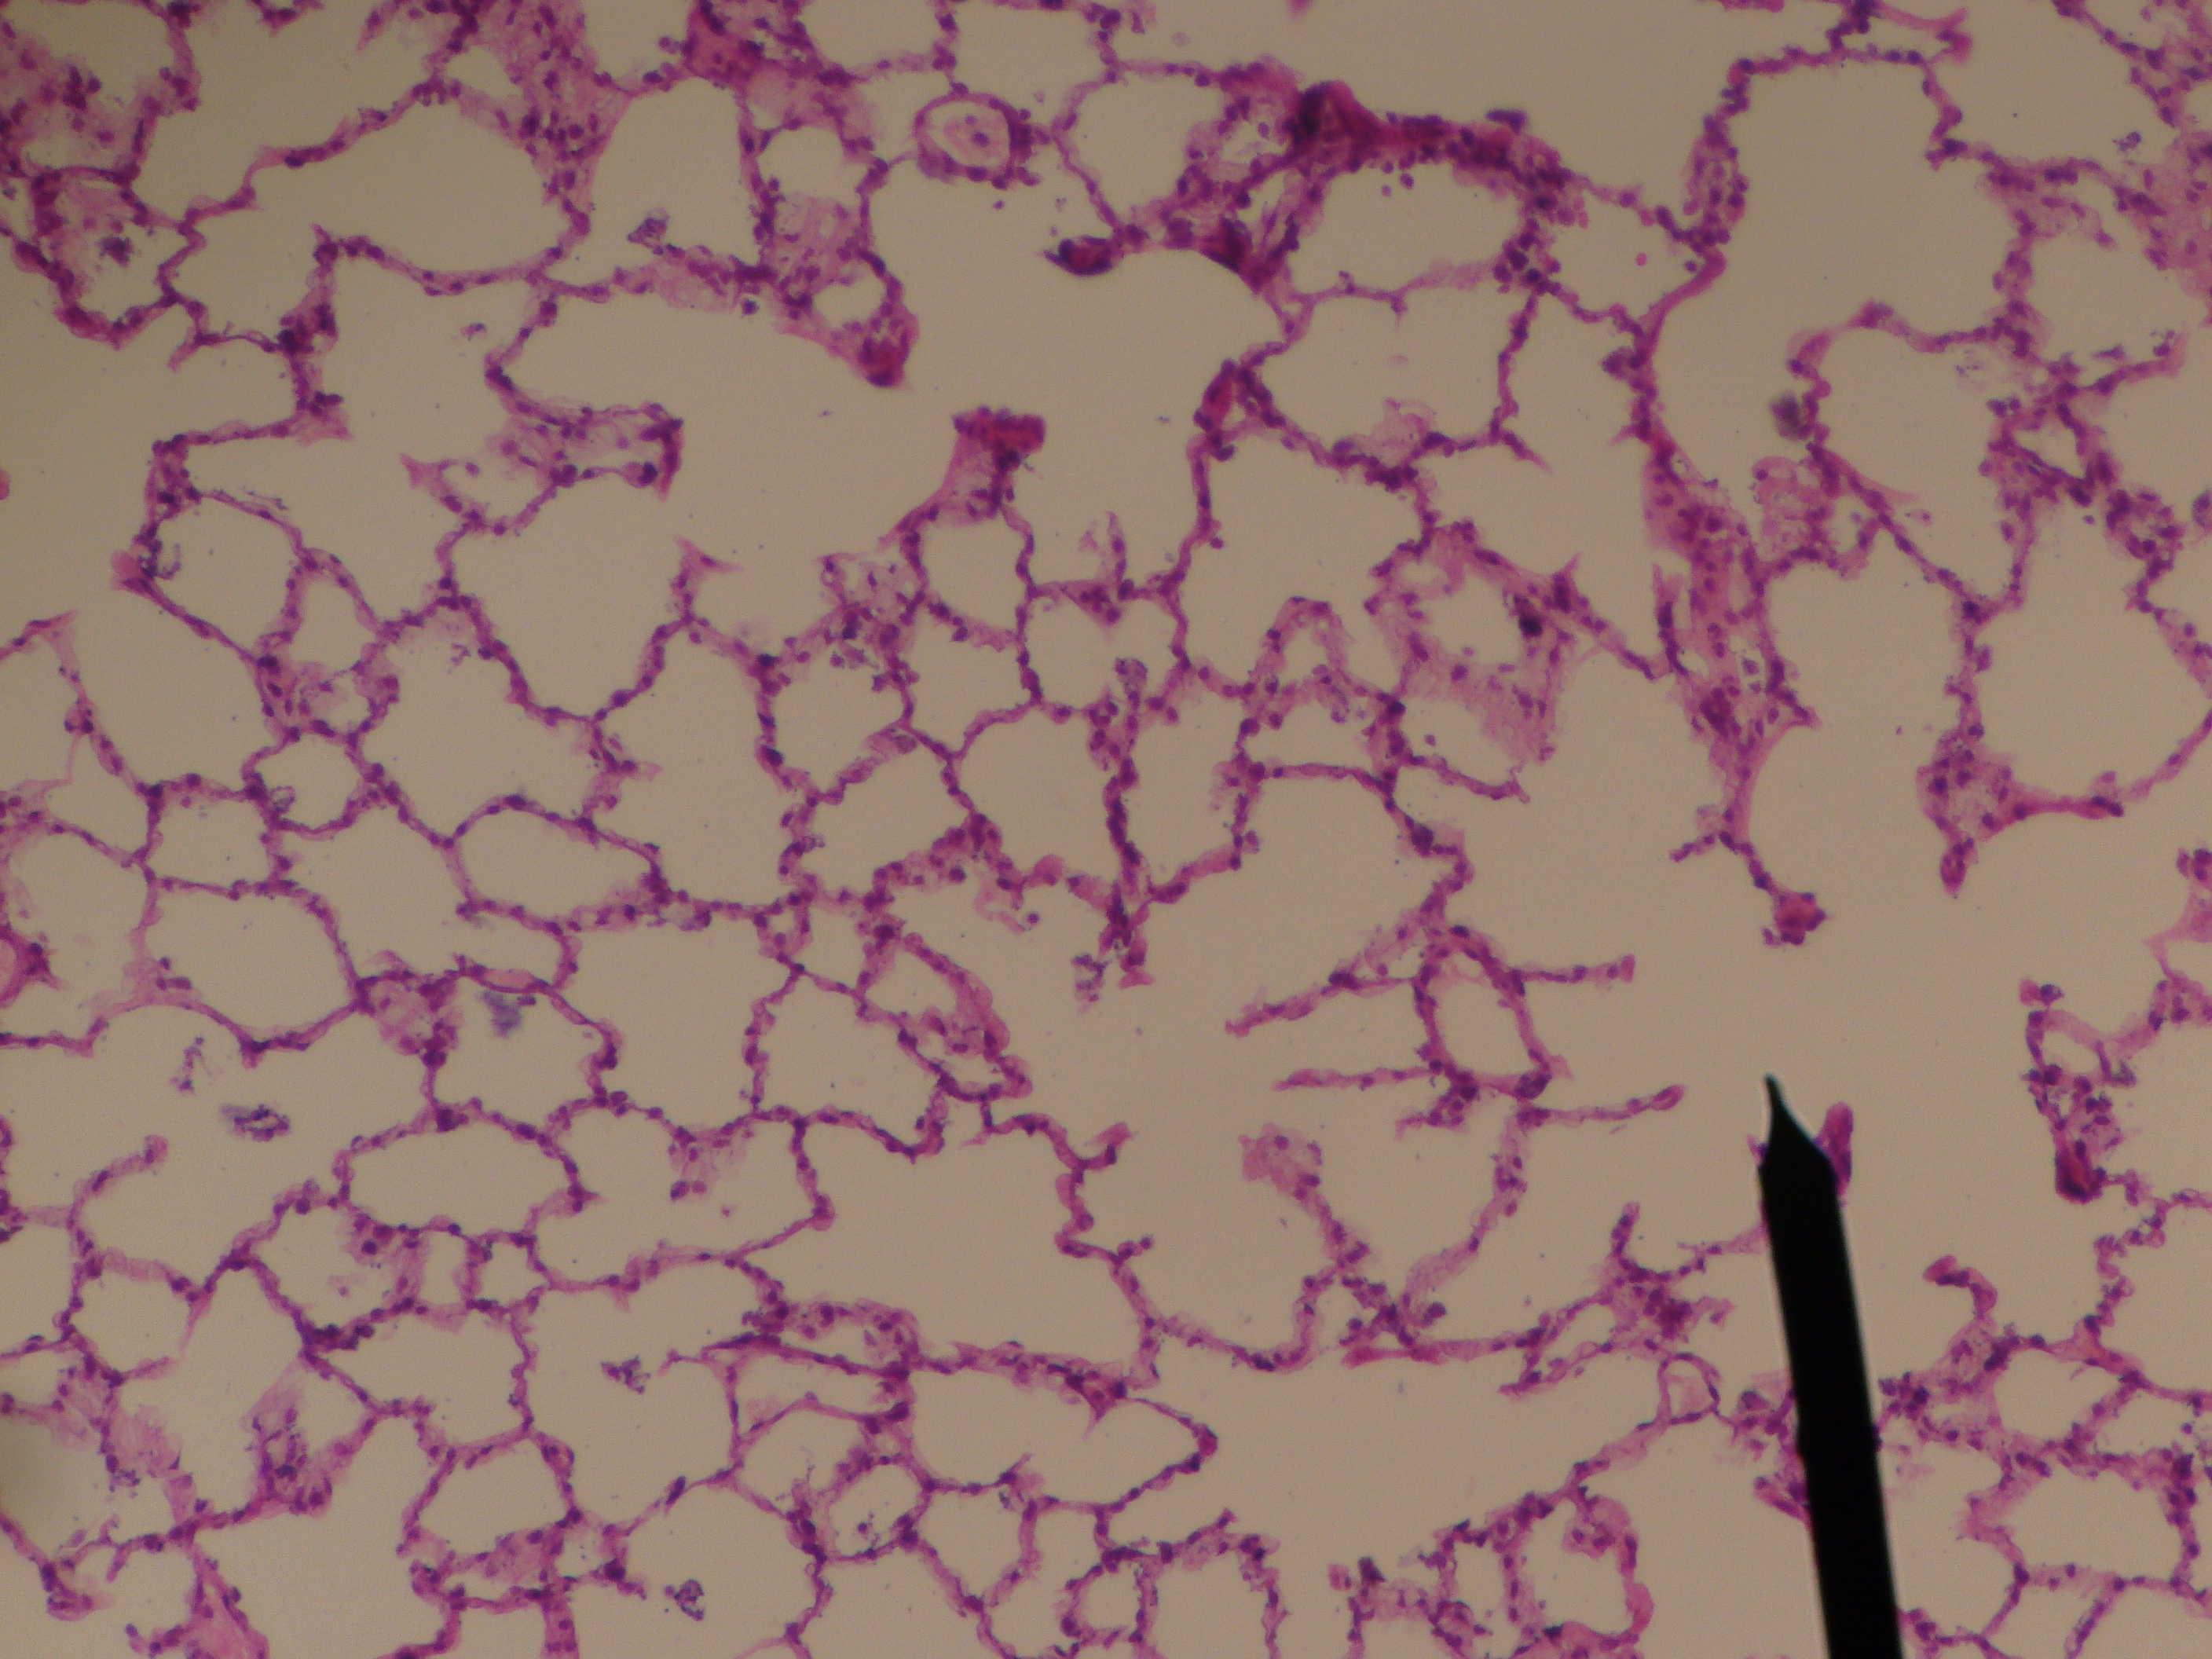
\includegraphics[width=\textwidth]{./figs/lung_figs/alveolar_sac}%
  \end{subfigure}
  ~
  \begin{subfigure}{0.5\textwidth}
    \begin{tikzpicture}%
      \node[anchor=south west,inner sep=0] (image) at (0,0) {
        \includegraphics[width=\textwidth]{./figs/lung_figs/lung_surface_alveoli}
      };%
      \begin{scope}[x={(image.south east)},y={(image.north west)}]%
        \node[left] at (1.0,0.95) {Soft tissue};%
        \node[left] at (1.0,0.38) {Lung surface};%
        \node[left] at (0.95,0.08) {\colorbox{gray!40}{Alveoli}};%
      \end{scope}%
      %
      \node[anchor=south west,inner sep=0] (image_wave) at (0.0,2.6) {
      \def\svgwidth{0.425\textwidth}\import{./figs/lung_figs/}{wave_only.pdf_tex}};%
      \draw[very thick] (1.3,1.7) -- (2.2,1.7) -- (2.2,2.5) -- (1.3,2.5) -- (1.3, 1.7); %
    \end{tikzpicture}%
  \end{subfigure}
  \caption[A histological cross section of alveoli.]{A histological
    cross section of alveoli (Left). A schematic of ultrasound
    impinging upon the lung surface and alveoli, from the surrounding
    soft tissue (Right). A black box surrounds an alveolar surface,
    which schematically illustrates the physical problem upon which
    the initial condition is created.[Alveolar cross section adapted
    from work by Jpogi [CC BY-SA 4.0
    (http://creativecommons.org/licenses/by-sa/4.0), via Wikimedia
    Commons]}%
  \label{fig:alveolar_histology}
\end{figure}%
% 
The diagnostic ultrasound pulse waveform, as illustrated in the time
domain in Figure \ref{fig:p0_ultrasound} is modeled as a sinusoidal
carrier wave of amplitude $p_a$ and frequency $f$ modulated by a
Gaussian Envelope, and as such that the initial pressure condition can
be described as,
\begin{align}
  p(y_f,t=0) = p_a\sin{\left(2\pi f\frac{y_f-L}{c}\right)}\exp{\left(-\frac{\left(\left[y_f-L/2\right]c\right)^2}{FWHM/\left(2\sqrt{2\ln{\left(2\right)}} \right)}\right)},%
\end{align}
where $y_f = y - 11a_0$ is the $y$-location, relative to the initial
location of the wave leading end. The carrier wavelength
$\lambda=c_{water}/f$ and the full width of the Gaussian envelope at
half of the maximum amplitude, or $FWHM$, are designed to scale
appropriately with respect to the alveolar length scale
$\ell=200~\mu$m. Here, we choose design parameters of
$f\approx 1.25 c / 2\pi \ell$ and $FWHM=15\ell$ such that the
corresponding center frequency is approximately $f=1.5$ MHz and
$FWHM=3$ mm. Accordingly, the pulse length $L=45\ell$ is defined such
that the pulse duration is approximately $6~\mu$s. In implementation
$L$ is the length of the computational domain, over which the wave is
defined to exist (i.e., pressure is set to ambient outside the wave
region, effectively truncating the ends of the Gaussian
envelope). This waveform is an analytical approximation of a true
\ac{DUS} pulse, which allows us to manipulate the parameters of
interest. %
\begin{figure}
  \centering \def\svgwidth{0.5\textwidth}
  \import{./figs/lung_figs/}{p0_vs_t_us_general.pdf_tex}%
  \caption[Ultrasound pulse waveform]{Ultrasound pulse waveform}
  \label{fig:p0_ultrasound}%
\end{figure}%

\subsection{Stress and strain at the alveolar interface}%
\label{subsec:usbe_lung_bio_stress_strain}
As previously mentioned, among the tissue layers surrounding the
alveoli are the pulmonary capillaries, a sheet-like, blood-filled web,
almost completely unsupported by surrounding tissue
\citep{West1991}. It is the hemorrhage of these capillaries that
interests us, and thus, to interpret the results of the numerical
experiments in the context of \ac{DUS}-induced lung hemorrhage, we
will calculate the linear strain and infer the viscous stress at the
liquid-gas interface, which represents the alveolar septa, where these
capillaries lie. We aim to compare the calculated stresses and strains
to relevant injury criteria. We note that from the available strain
and strain rate data, it would be possible to infer a total
viscoelastic stress at the interface if a constitutive model were
known. However, constitutive models appropriate to this work do not
appear available at this time and the development of such models would
require experiments far beyond the scope of this work.%
\begin{comment}
  For sake of justification of the model, a simple model for
  estimating the order of magnitude of the involved elastic forces can
  be found in \ref{app:lung_elastic}
\end{comment}

\paragraph*{Calculation of the viscous stress}
Viscous stresses resist motion of the flow, however since the Euler
equations, which are inherently inviscid, are solved, we aim to infer
the viscous stress resulting from the interfacial motion and
deformation. We do this because, while the justifications in Chapter
\ref{ch:usbe_lung} suggest that flow dynamics can be reasonably
approximated by neglecting viscosity an understanding of the
approximate viscous stress associated with \ac{DUS} is necessary to
understand the results in the context of alveolar injury. To do this
we infer the viscosity at each point in space and time as $\mu(x,y,t)$
based on the physical properties of air and water, and the volume
fraction of water $\alpha(x,y,t)$ given that
$\mu = \alpha\mu_{water} + (1-\alpha)\mu_{air}$. The shear stress in a
two-dimensional, Newtonian flow is calculated using the computed
viscosity field and the velocity gradients as
\begin{align}
  \tau_{xy}(x,y,t) = \mu\left(\frac{\partial u}{\partial y}+ \frac{\partial v}{\partial x}\right),
\end{align}
where $u$ and $v$ represent the $x$- and $y$-components of the
velocity. The maximum viscous stress amplitude is extracted from the
field at each point in time from our simulations.
% 
\begin{comment}
  \begin{align}%
    \tau_{ij}=\mu%
    \begin{bmatrix}%
      0 & \frac{\partial u}{\partial y}+\frac{\partial v}{\partial x}\\%
      \frac{\partial v}{\partial x}+\frac{\partial u}{\partial y} & 0%
    \end{bmatrix}%
  \end{align},
\end{comment}
% 
\paragraph*{Calculation of the interface strain}
The linear interfacial strain is calculated as
\begin{align}%
  \label{eq:linear_strain}%
  \varepsilon = \frac{s(t) - s_0}{s_0}
\end{align}
where $s(t)$ is the arc length of the interface, which is initially
$s_0=s(0)$.  While some of the large deformations we observe in our
results may actually be out of the realm of finite strain, we choose
this metric, which is consistent with previous alveolar strain
calculations in the literature. For example, \cite{Roan2011} used the
relative change in alveolar diameters, which is analogous to relative
change in the interface arc length here.
\begin{comment}
  \cite{Perlman2014} combined experimentally measured strains with
  computationally modeled lung stresses to demonstrate that the
  effective Young's moduli of alveolar septa depend on transpulmonary
  pressure. Values range from a minimum of $E_a=12$ kPa in the low
  transpulmonary pressure range of $\approx 0.4$-$0.6$ kPa to a
  maximum $E_a=140$ kPa at a high transpulmonary pressure of range,
  $\approx 1.5$-$2.5$ kPa.
\end{comment}

%%%%%%%%%%%%%%%%%%%%%%%%%%%%%%% 
\section{Results and Discussion}
To accomplish the aims of this study, two sets of numerical
experiments are performed. The first set of experiments is designed to
determine the stresses and strains on a perturbed liquid-gas
interface, driven by clinically relevant ultrasound
pulses. Simulations of interactions between sinusoidally perturbed
water-air interfaces and diagnostic ultrasound pulses are performed
for wave amplitudes of $p_a=1.0$, $2.5$, and $5.0$ MPa and initial
perturbation amplitudes of $a_0=0.03\ell$, $0.10\ell$ and
$0.30\ell$. The second set of experiments is designed to test the
hypothesis that \ac{US} pulses are capable of generating sufficient
baroclinic vorticity at an air-water interface to drive appreciable
interface deformation. For this second set of experiments, which is
described in greater detail in Section
\ref{subsec:vorticity_experiments}, we perform simulations of an
\ac{US} pulse-driven gas-liquid interface, with parameters similar to
those of the baseline trapezoidal wave in Chapter \ref{ch:usbe_lung}
($p_a = 10$ MPa, $a_0 = 0.03\ell$, $L=45\ell$) and compare interface
growth dynamics driven by a \ac{US} pulse to those driven by the
trapezoidal wave of Chapter \ref{ch:usbe_lung}.

\subsection{Qualitative observations of the interface}
To illustrate the evolution of the interface, Figures
\ref{fig:rho_snapshots_A10}, \ref{fig:rho_snapshots_A25}, and
\ref{fig:rho_snapshots_A50} show density contours for pulse amplitudes
of $1.0, 2.5,$ and $5.0$ MPa, respectively, at dimensionless times
$t/(\ell/c)=4.75, 47.5, 475,$ and $2374$. While these dimensionless
quantities are used for comparison of this work to that of Chapter
\ref{ch:usbe_lung}, for the sake of physicality, we will report times
and stresses in this section as dimensional quantities. As such, for
an $\ell = 200~\mu$m alveolar diameter, these dimensionless times
approximately corresponds to dimensional times of $0.6, 6.0, 60,$ and
$290~\mu$s. In each case, subfigures \subref{fig:rho_snapshot_03},
\subref{fig:rho_snapshot_10}, and \subref{fig:rho_snapshot_30}
correspond to initial perturbation amplitudes of
$a_0=0.03\ell, 0.10\ell,$ and $0.30\ell$ respectively; $t = 0.6~ \mu$s
occurs just after the wave first encounters the interface and by
$t= 6.0~ \mu$s the wave has completely passed. For the $p_a = 1.0$ MPa
pulse, the interface remains largely unmoved and undeformed by the
interaction with the wave, even at late times (illustrated in Figure
\ref{fig:rho_snapshots_A10}). For the $p_a = 2.5$ MPa pulse, little
deformation is observed for $a_0 = 0.03\ell$, however at higher
initial amplitudes ($a_0 = 0.10\ell$ and $0.30\ell$), the interface is
clearly deformed at late times and a cusp is observed to form along
the interface at $x/\ell = 0.5$ (illustrated in Figure
\ref{fig:rho_snapshots_A25}). For the $p_a = 5.0$ MPa pulse, obvious
deformation is observed for all considered values of $a_0$
(illustrated in Figure \ref{fig:rho_snapshots_A50}). For
$a_0 = 0.10\ell$ and $0.30\ell$, a spike of heavy fluid with a cusp at
$x = 0.5$ is again observed to form at late times.  For all incoming
waves, the degree of deformation appears to increase with increasing
initial perturbation amplitude $a_0$ and wave amplitude $p_a$. The
observed sharp features, which evolved from an initially smooth
interface perturbation, could potentially lead to stress concentration,
which in alveoli, may lead to hemorrhage.
% 
\definecolor{airgray}{HTML}{DDDDDD}
\begin{figure}
  \vspace*{-0.5cm}
  \centering
  \begin{subfigure}[b]{0.9\textwidth}
    \begin{tikzpicture}%
      \node[anchor=south west,inner sep=0] (image) at (0,0) {
        \includegraphics[width=\textwidth]{./figs/lung_figs/rmawave_1_A10_a03_t500_rho_snapshots_printable}
      };%
      \begin{scope}[x={(image.south east)},y={(image.north west)}]%
        \node[font=\small,right] at (0.06,0.9) {\textcolor{white}{$\rho(x,y)$}};%
        \node[font=\small,right] at (0.7,0.9) {\textcolor{white}{(a) $a_0=0.03\ell$}};%
        \node[font=\small,right] at (0.06,0.14) {\colorbox{airgray}{$t = 0.6~\mu$s}};% t/(\ell c_{air})=1
        \node[font=\small,right] at (0.26,0.14) {\colorbox{airgray}{$t = 6.0~\mu$s\quad}};%t/(\ell c_{air})=10
        \node[font=\small,right] at (0.475,0.14) {\colorbox{airgray}{$t = 60~\mu$s\quad}};%t/(\ell c_{air})=100
        \node[font=\small,right] at (0.685,0.14) {\colorbox{airgray}{$t = 288~\mu$s\quad}};%t/(\ell c_{air})=500
      \end{scope}%  
      % \begin{scope}[x={(image.south east)},y={(image.north west)}]%
      %   \node[font=\small,right] at (0.06,0.9) {\textcolor{white}{$\rho(x,y)$}};%
      %   \node[font=\small,right] at (0.06,0.14) {\colorbox{airgray}{$t = 1 $ ($0.6~\mu$s)}};%
      %   \node[font=\small,right] at (0.26,0.14) {\colorbox{airgray}{$t = 10 $ ($6.0~\mu$s)}};%
      %   \node[font=\small,right] at (0.475,0.14) {\colorbox{airgray}{$t = 100 $ ($60.0~\mu$s)}};%
      %   \node[font=\small,right] at (0.685,0.14) {\colorbox{airgray}{$t = 300 $ ($500.0\mu$s)}};%
      % \end{scope}%  
    \end{tikzpicture}%
    \phantomcaption
    \label{fig:rho_snapshot_03}
    % \caption{\label{fig:rho_snapshot_03} $a_0 = 0.03\ell$}
  \end{subfigure}
  % 
  \begin{subfigure}[b]{0.9\textwidth}
    \begin{tikzpicture}%
      \node[anchor=south west,inner sep=0] (image) at (0,0) {
        \includegraphics[width=\textwidth]{./figs/lung_figs/rmawave_1_A10_a10_t500_rho_snapshots}
      };%
      \begin{scope}[x={(image.south east)},y={(image.north west)}]%
        \node[font=\small,right] at (0.06,0.9) {\textcolor{white}{$\rho(x,y)$}};%
        \node[font=\small,right] at (0.7,0.9) {\textcolor{white}{(b) $a_0=0.10\ell$}};%
        \node[font=\small,right] at (0.06,0.14) {\colorbox{airgray}{$t = 0.6~\mu$s}};% t/(\ell c_{air})=1
        \node[font=\small,right] at (0.26,0.14) {\colorbox{airgray}{$t = 6.0~\mu$s\quad}};%t/(\ell c_{air})=10
        \node[font=\small,right] at (0.475,0.14) {\colorbox{airgray}{$t = 60~\mu$s\quad}};%t/(\ell c_{air})=100
        \node[font=\small,right] at (0.685,0.14) {\colorbox{airgray}{$t = 288~\mu$s\quad}};%t/(\ell c_{air})=500
      \end{scope}%  
    \end{tikzpicture}%
    \phantomcaption
    \label{fig:rho_snapshot_10}
    % \caption{\label{fig:rho_snapshot_10} $a_0 = 0.10\ell$}
  \end{subfigure}
  % 
  \begin{subfigure}[b]{0.9\textwidth}
    \begin{tikzpicture}%
      \node[anchor=south west,inner sep=0] (image) at (0,0) {
        \includegraphics[width=\textwidth]{./figs/lung_figs/rmawave_1_A10_a30_t500_rho_snapshots}
      };%
      \begin{scope}[x={(image.south east)},y={(image.north west)}]%
        \node[font=\small,right] at (0.06,0.9) {\textcolor{white}{$\rho(x,y)$}};%
        \node[font=\small,right] at (0.7,0.9) {\textcolor{white}{(c) $a_0=0.30\ell$}};%
        \node[font=\small,right] at (0.06,0.14) {\colorbox{airgray}{$t = 0.6~\mu$s\quad}};% t/(\ell c_{air})=1
        \node[font=\small,right] at (0.26,0.14) {\colorbox{airgray}{$t = 6.0~\mu$s\quad}};%t/(\ell c_{air})=10
        \node[font=\small,right] at (0.475,0.14) {\colorbox{airgray}{$t = 60~\mu$s\quad}};%t/(\ell c_{air})=100
        \node[font=\small,right] at (0.685,0.14) {\colorbox{airgray}{$t = 288~\mu$s\quad}};%t/(\ell c_{air})=500
      \end{scope}%  
    \end{tikzpicture}%
    \phantomcaption
    \label{fig:rho_snapshot_30}
    % \caption{\label{fig:rho_snapshot_30} $a_0 = 0.30\ell$}
  \end{subfigure}
  \caption[Evolution of the interface for $p_a=1.0$ MPa ultrasound
  wave]{Evolution of the interface for $p_a=1.0$ MPa ultrasound
    wave. Density contours at $t=0.6, 6.0, 60,$ and $288~\mu$s for
    initial perturbation amplitudes \subref{fig:rho_snapshot_03}
    $a_0 = 0.03\ell$, \subref{fig:rho_snapshot_10} $a_0 = 0.10\ell$,
    and \subref{fig:rho_snapshot_30} $a_0 = 0.30\ell$.}
  \label{fig:rho_snapshots_A10}
\end{figure}
% 
% 
\begin{figure}
  \vspace*{-0.5cm}
  \centering
  \begin{subfigure}[b]{0.9\textwidth}
    % \includegraphics[width=\textwidth]{./figs/lung_figs/rmawave_1_A25_a03_t500_rho_snapshots}
    \begin{tikzpicture}%
      \node[anchor=south west,inner sep=0] (image) at (0,0) {
        \includegraphics[width=\textwidth]{./figs/lung_figs/rmawave_1_A25_a03_t500_rho_snapshots_printable}
      };%
      \begin{scope}[x={(image.south east)},y={(image.north west)}]%
        \node[font=\small,right] at (0.06,0.9) {\textcolor{white}{$\rho(x,y)$}};%
        \node[font=\small,right] at (0.7,0.9) {\textcolor{white}{(a) $a_0=0.03\ell$}};%
        \node[font=\small,right] at (0.06,0.14) {\colorbox{airgray}{$t = 0.6~\mu$s\quad}};% t/(\ell c_{air})=1
        \node[font=\small,right] at (0.26,0.14) {\colorbox{airgray}{$t = 6.0~\mu$s\quad}};%t/(\ell c_{air})=10
        \node[font=\small,right] at (0.475,0.14) {\colorbox{airgray}{$t = 60~\mu$s\quad}};%t/(\ell c_{air})=100
        \node[font=\small,right] at (0.685,0.14) {\colorbox{airgray}{$t = 288~\mu$s\quad}};%t/(\ell c_{air})=500
      \end{scope}%  
    \end{tikzpicture}%
    \caption{\label{fig:rho_snapshot_A25_a03} $a_0 = 0.03\ell$}
  \end{subfigure}
  % 
  \begin{subfigure}[b]{0.9\textwidth}

    \begin{tikzpicture}%
      \node[anchor=south west,inner sep=0] (image) at (0,0) {
        \includegraphics[width=\textwidth]{./figs/lung_figs/rmawave_1_A25_a10_t500_rho_snapshots_printable}
      };%
      \begin{scope}[x={(image.south east)},y={(image.north west)}]%
        \node[font=\small,right] at (0.06,0.9) {\textcolor{white}{$\rho(x,y)$}};%
        \node[font=\small,right] at (0.7,0.9) {\textcolor{white}{(b) $a_0=0.10\ell$}};%
        \node[font=\small,right] at (0.06,0.14) {\colorbox{airgray}{$t = 0.6~ \mu$s}};% t/(\ell c_{air})=1
        \node[font=\small,right] at (0.26,0.14) {\colorbox{airgray}{$t = 6.0~ \mu$s\quad}};%t/(\ell c_{air})=10
        \node[font=\small,right] at (0.475,0.14) {\colorbox{airgray}{$t = 60~ \mu$s\quad}};%t/(\ell c_{air})=100
        \node[font=\small,right] at (0.685,0.14) {\colorbox{airgray}{$t = 288~ \mu$s\quad}};%t/(\ell c_{air})=500
      \end{scope}%  
    \end{tikzpicture}%
    \phantomcaption
    \label{fig:rho_snapshot_A25_a10}
  \end{subfigure}
  % 
  \begin{subfigure}[b]{0.9\textwidth}
    \begin{tikzpicture}%
      \node[anchor=south west,inner sep=0] (image) at (0,0) {
        \includegraphics[width=\textwidth]{./figs/lung_figs/rmawave_1_A25_a30_t500_rho_snapshots_printable}
      };%
      \begin{scope}[x={(image.south east)},y={(image.north west)}]%
        \node[font=\small,right] at (0.06,0.9) {\textcolor{white}{$\rho(x,y)$}};%
        \node[font=\small,right] at (0.7,0.9) {\textcolor{white}{(c) $a_0=0.30\ell$}};%
        \node[font=\small,right] at (0.06,0.14) {\colorbox{airgray}{$t = 0.6~ \mu$s\quad}};% t/(\ell c_{air})=1
        \node[font=\small,right] at (0.26,0.14) {\colorbox{airgray}{$t = 6.0~ \mu$s\quad}};%t/(\ell c_{air})=10
        \node[font=\small,right] at (0.475,0.14) {\colorbox{airgray}{$t = 60~ \mu$s\quad}};%t/(\ell c_{air})=100
        \node[font=\small,right] at (0.685,0.14) {\colorbox{airgray}{$t = 288~ \mu$s\quad}};%t/(\ell c_{air})=500
      \end{scope}%  
    \end{tikzpicture}%
    \phantomcaption
    \label{fig:rho_snapshot_A25_a30}
  \end{subfigure}
  % 
  \caption[Evolution of the interface for $p_a=2.5$ MPa ultrasound
  wave]{Evolution of the interface for $p_a=2.5$ MPa ultrasound
    wave. Density contours at $t=0.6, 6.0, 60,$ and $288~\mu$s for initial
    perturbation amplitudes \subref{fig:rho_snapshot_03}
    $a_0 = 0.03\ell$, \subref{fig:rho_snapshot_10} $a_0 = 0.10\ell$,
    and \subref{fig:rho_snapshot_30} $a_0 = 0.30\ell$.}
  \label{fig:rho_snapshots_A25}
\end{figure}
% 
\begin{figure}
  \vspace*{-0.5cm}
  \centering
  \begin{subfigure}[b]{0.9\textwidth}
    \begin{tikzpicture}%
      \node[anchor=south west,inner sep=0] (image) at (0,0) {
        \includegraphics[width=\textwidth]{./figs/lung_figs/rmawave_1_A50_a03_t500_rho_snapshots}
      };%
      \begin{scope}[x={(image.south east)},y={(image.north west)}]%
        \node[font=\small,right] at (0.06,0.9) {\textcolor{white}{$\rho(x,y)$}};%
        \node[font=\small,right] at (0.7,0.9) {\textcolor{white}{(a) $a_0=0.03\ell$}};%
        \node[font=\small,right] at (0.06,0.14) {\colorbox{airgray}{$t = 0.6~\mu$s\quad}};% t/(\ell c_{air})=1
        \node[font=\small,right] at (0.26,0.14) {\colorbox{airgray}{$t = 6.0~\mu$s\quad}};%t/(\ell c_{air})=10
        \node[font=\small,right] at (0.475,0.14) {\colorbox{airgray}{$t = 60~\mu$s\quad}};%t/(\ell c_{air})=100
        \node[font=\small,right] at (0.685,0.14) {\colorbox{airgray}{$t = 288~\mu$s\quad}};%t/(\ell c_{air})=500
      \end{scope}%  
    \end{tikzpicture}%
    \caption{\label{fig:rho_snapshot_A50_a03} $a_0 = 0.03\ell$}
  \end{subfigure}
  % 
  \begin{subfigure}[b]{0.9\textwidth}
    \begin{tikzpicture}%
      \node[anchor=south west,inner sep=0] (image) at (0,0) {
        \includegraphics[width=\textwidth]{./figs/lung_figs/rmawave_1_A50_a10_t500_rho_snapshots}
      };%
      \begin{scope}[x={(image.south east)},y={(image.north west)}]%
        \node[font=\small,right] at (0.06,0.9) {\textcolor{white}{$\rho(x,y)$}};%
        \node[font=\small,right] at (0.7,0.9) {\textcolor{white}{(b) $a_0=0.10\ell$}};%
        \node[font=\small,right] at (0.06,0.14) {\colorbox{airgray}{$t = 0.6~\mu$s\quad}};% t/(\ell c_{air})=1
        \node[font=\small,right] at (0.26,0.14) {\colorbox{airgray}{$t = 6.0~\mu$s\quad}};%t/(\ell c_{air})=10
        \node[font=\small,right] at (0.475,0.14) {\colorbox{airgray}{$t = 60~\mu$s\quad}};%t/(\ell c_{air})=100
        \node[font=\small,right] at (0.685,0.14) {\colorbox{airgray}{$t = 288~\mu$s\quad}};%t/(\ell c_{air})=500
      \end{scope}%  
    \end{tikzpicture}%
    \caption{\label{fig:rho_snapshot_A50_a10} $a_0 = 0.10\ell$}
  \end{subfigure}
  % 
  \begin{subfigure}[b]{0.9\textwidth}
    \begin{tikzpicture}%
      \node[anchor=south west,inner sep=0] (image) at (0,0) {
        \includegraphics[width=\textwidth]{./figs/lung_figs/rmawave_1_A50_a30_t500_rho_snapshots}
      };%
      \begin{scope}[x={(image.south east)},y={(image.north west)}]%
        \node[font=\small,right] at (0.06,0.9) {\textcolor{white}{$\rho(x,y)$}};%
        \node[font=\small,right] at (0.7,0.9) {\textcolor{white}{(c) $a_0=0.30\ell$}};%
        \node[font=\small,right] at (0.06,0.14) {\colorbox{airgray}{$t = 0.6~\mu$s\quad}};% t/(\ell c_{air})=1
        \node[font=\small,right] at (0.26,0.14) {\colorbox{airgray}{$t = 6.0~\mu$s\quad}};%t/(\ell c_{air})=10
        \node[font=\small,right] at (0.475,0.14) {\colorbox{airgray}{$t = 60~\mu$s\quad}};%t/(\ell c_{air})=100
        \node[font=\small,right] at (0.685,0.14) {\colorbox{airgray}{$t = 288~\mu$s\quad}};%t/(\ell c_{air})=500
      \end{scope}%  
    \end{tikzpicture}%
    \caption{\label{fig:rho_snapshot_A50_a30} $a_0 = 0.30\ell$}
  \end{subfigure}
  % 
  \caption[Evolution of the interface for $p_a=5.0$ MPa ultrasound
  wave]{Evolution of the interface for $p_a=5.0$ MPa ultrasound
    wave. Density contours at $t=0.6, 6.0, 60,$ and $288~\mu$s for
    initial perturbation amplitudes \subref{fig:rho_snapshot_03}
    $a_0 = 0.03\ell$, \subref{fig:rho_snapshot_10} $a_0 = 0.10\ell$,
    and \subref{fig:rho_snapshot_30} $a_0 = 0.30\ell$.}
  \label{fig:rho_snapshots_A50}
\end{figure}
\subsection{Interface strain, $\varepsilon$}
In consideration of possible strain-related damage of the alveolar
wall we examine the linear interface strain $\varepsilon(t)$, as
defined in Equation \eqref{eq:linear_strain}, and its dependence on
wave amplitude $p_a$ and perturbation amplitude $a_0$. Figure
\ref{fig:pa_dependence_strain} shows strain histories $\varepsilon(t)$
for variable $p_a = 1.0$ (blue), $2.5$ (red), and $5.0$ (green) MPa
and constant initial perturbation amplitude $a_0=0.03\ell$
\subref{fig:strain_multi-pa_a03}, $0.10\ell$
\subref{fig:strain_multi-pa_a10}, and $0.30\ell$
\subref{fig:strain_multi-pa_a30}, while Figure
\ref{fig:a0_dependence_strain} shows these data re-plotted for
variable $a_0 = 0.03\ell$ (blue), $0.10\ell$ (red), and $0.30\ell$
(green) and constant wave amplitudes $p_a=1.0$
\subref{fig:strain_multi-a0-A10}, $2.5$
\subref{fig:strain_multi-a0-A25}, and $5.0$
\subref{fig:strain_multi-a0-A50} MPa. For all pressure amplitudes
$p_a$ and initial perturbation amplitudes $a_0$, negative strain is
observed during and immediately following the wave-interface
interaction, indicating a net reduction in interfacial length. This
reduction is observed to correspond to the flattening of the interface
perturbation during and after the interaction with the acoustic
pulse. For the $p_a = 1.0$ MPa wave with all $a_0$ and the $2.5$ MPa
wave with $a_0 = 0.03\ell$ and $0.10\ell$, this reduction in interface
length is observed to slowly continue at a decreasing rate throughout
the duration of the simulation. For the $p_a = 2.5$ MPa wave with
$a_0 = 0.30\ell$ and the $p_a = 5.0$ MPa wave with all $a_0$, a
stretching or increase in interfacial length follows the length
reduction. Based on Figures \ref{fig:rho_snapshots_A25} and
\ref{fig:rho_snapshots_A50}, the increased interfacial length
corresponds to the growth of the liquid spike into the gas. It is
observed that this deformation and strain increase takes place long
after the passage of the wave, when the acoustic pressure is
negligible $\left(t/(\ell/c)\gtrsim 47.5\right)$. As explained in
Chapter \ref{ch:usbe_lung}, the deformation cannot be explained by
linear acoustics, which predicts negligible deformation after the
passage of the wave.

The interface strains increase with increasing $p_a$ and $a_0$, which
is consistent with baroclinic vorticity-driven growth because these
quantities determine the wave pressure gradient and its degree of
misalignment with interface density gradient. The minimal strain case
is observed for the smallest considered initial perturbation and wave
amplitudes ($a_0 = 0.03\ell$, $p_a = 1.0$ MPa), for which a maximum
strain amplitude of $\varepsilon=0.001$ was observed at the final
computed time $t = 288~\mu$s. Conversely, the maximum strain case
occurs for the largest considered initial perturbation and wave
amplitudes ($a_0 = 0.30\ell$, $p_a = 5.0$ MPa), for which, a maximum
strain amplitude of $\varepsilon=0.38$ was observed at the final
computed time $t = 288 ~\mu$s. We highlight that for the $p_a=5.0$ MPa
case, these are not small strains and linear strain theory is not
likely to apply, even if failure of the interface has not yet
occurred. We consider the strain results relative to the
$\varepsilon=0.08$ strain failure criteria \citep{Belete2010}. Over
the simulated duration, this threshold was exceeded only for the
$p_a = 5.0$ MPa wave with $a_0 \geq 0.10\ell$ and $0.30\ell$, in which
cases the strain exceeded $\varepsilon=0.08$ at approximately $t=100$
and $220~\mu$s respectively.
% 
\begin{figure}
  \centering
  \begin{subfigure}[b]{0.49\textwidth}
    % 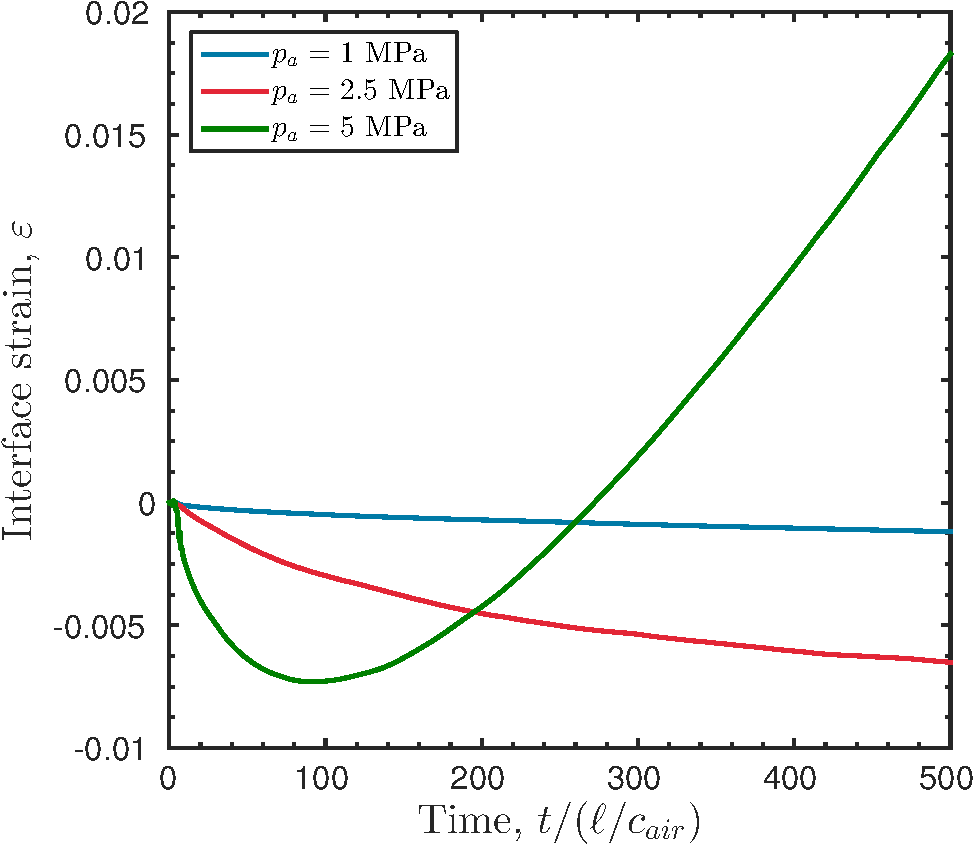
\includegraphics[width=\textwidth]{./figs/lung_figs/rmawave_1_A10,25,50_a03_strain_08-Mar-2017}
    \includegraphics[width=\textwidth]{./figs/lung_figs/rmawave_1_A10,25,50_a03_strain_15-Jun-2017_dim}
    \caption{\label{fig:strain_multi-pa_a03} $a_0 = 0.03\ell$}
  \end{subfigure}
  ~ 
  \begin{subfigure}[b]{0.49\textwidth}
    % 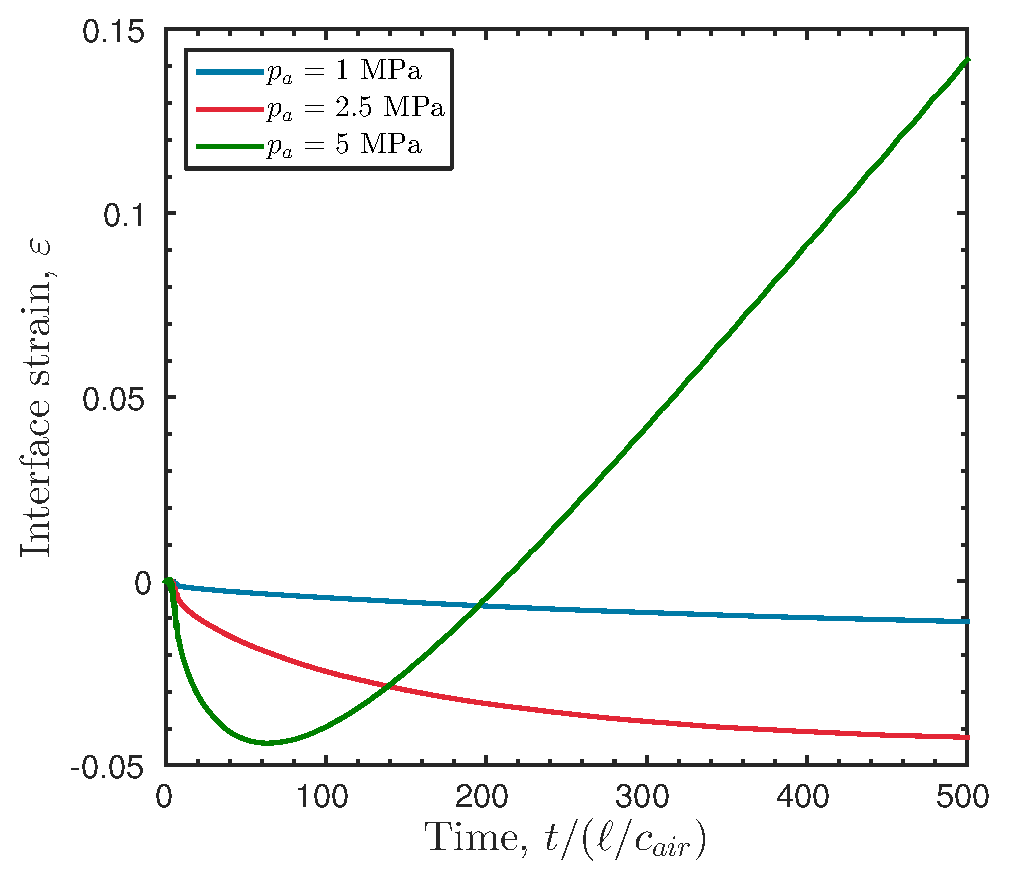
\includegraphics[width=\textwidth]{./figs/lung_figs/rmawave_1_A10,25,50_a10_strain_08-Mar-2017}
    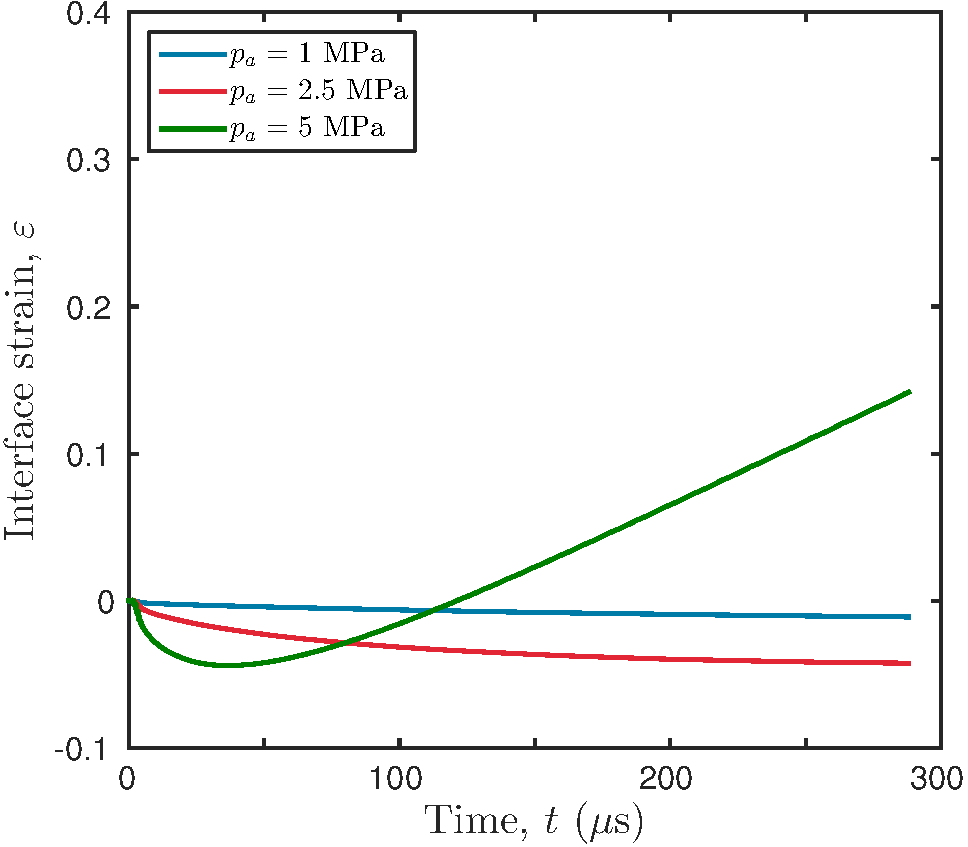
\includegraphics[width=\textwidth]{./figs/lung_figs/rmawave_1_A10,25,50_a10_strain_15-Jun-2017_dim}
    \caption{\label{fig:strain_multi-pa_a10} $a_0 = 0.10\ell$}
  \end{subfigure}
  ~ 
  \begin{subfigure}[b]{0.49\textwidth}
    % 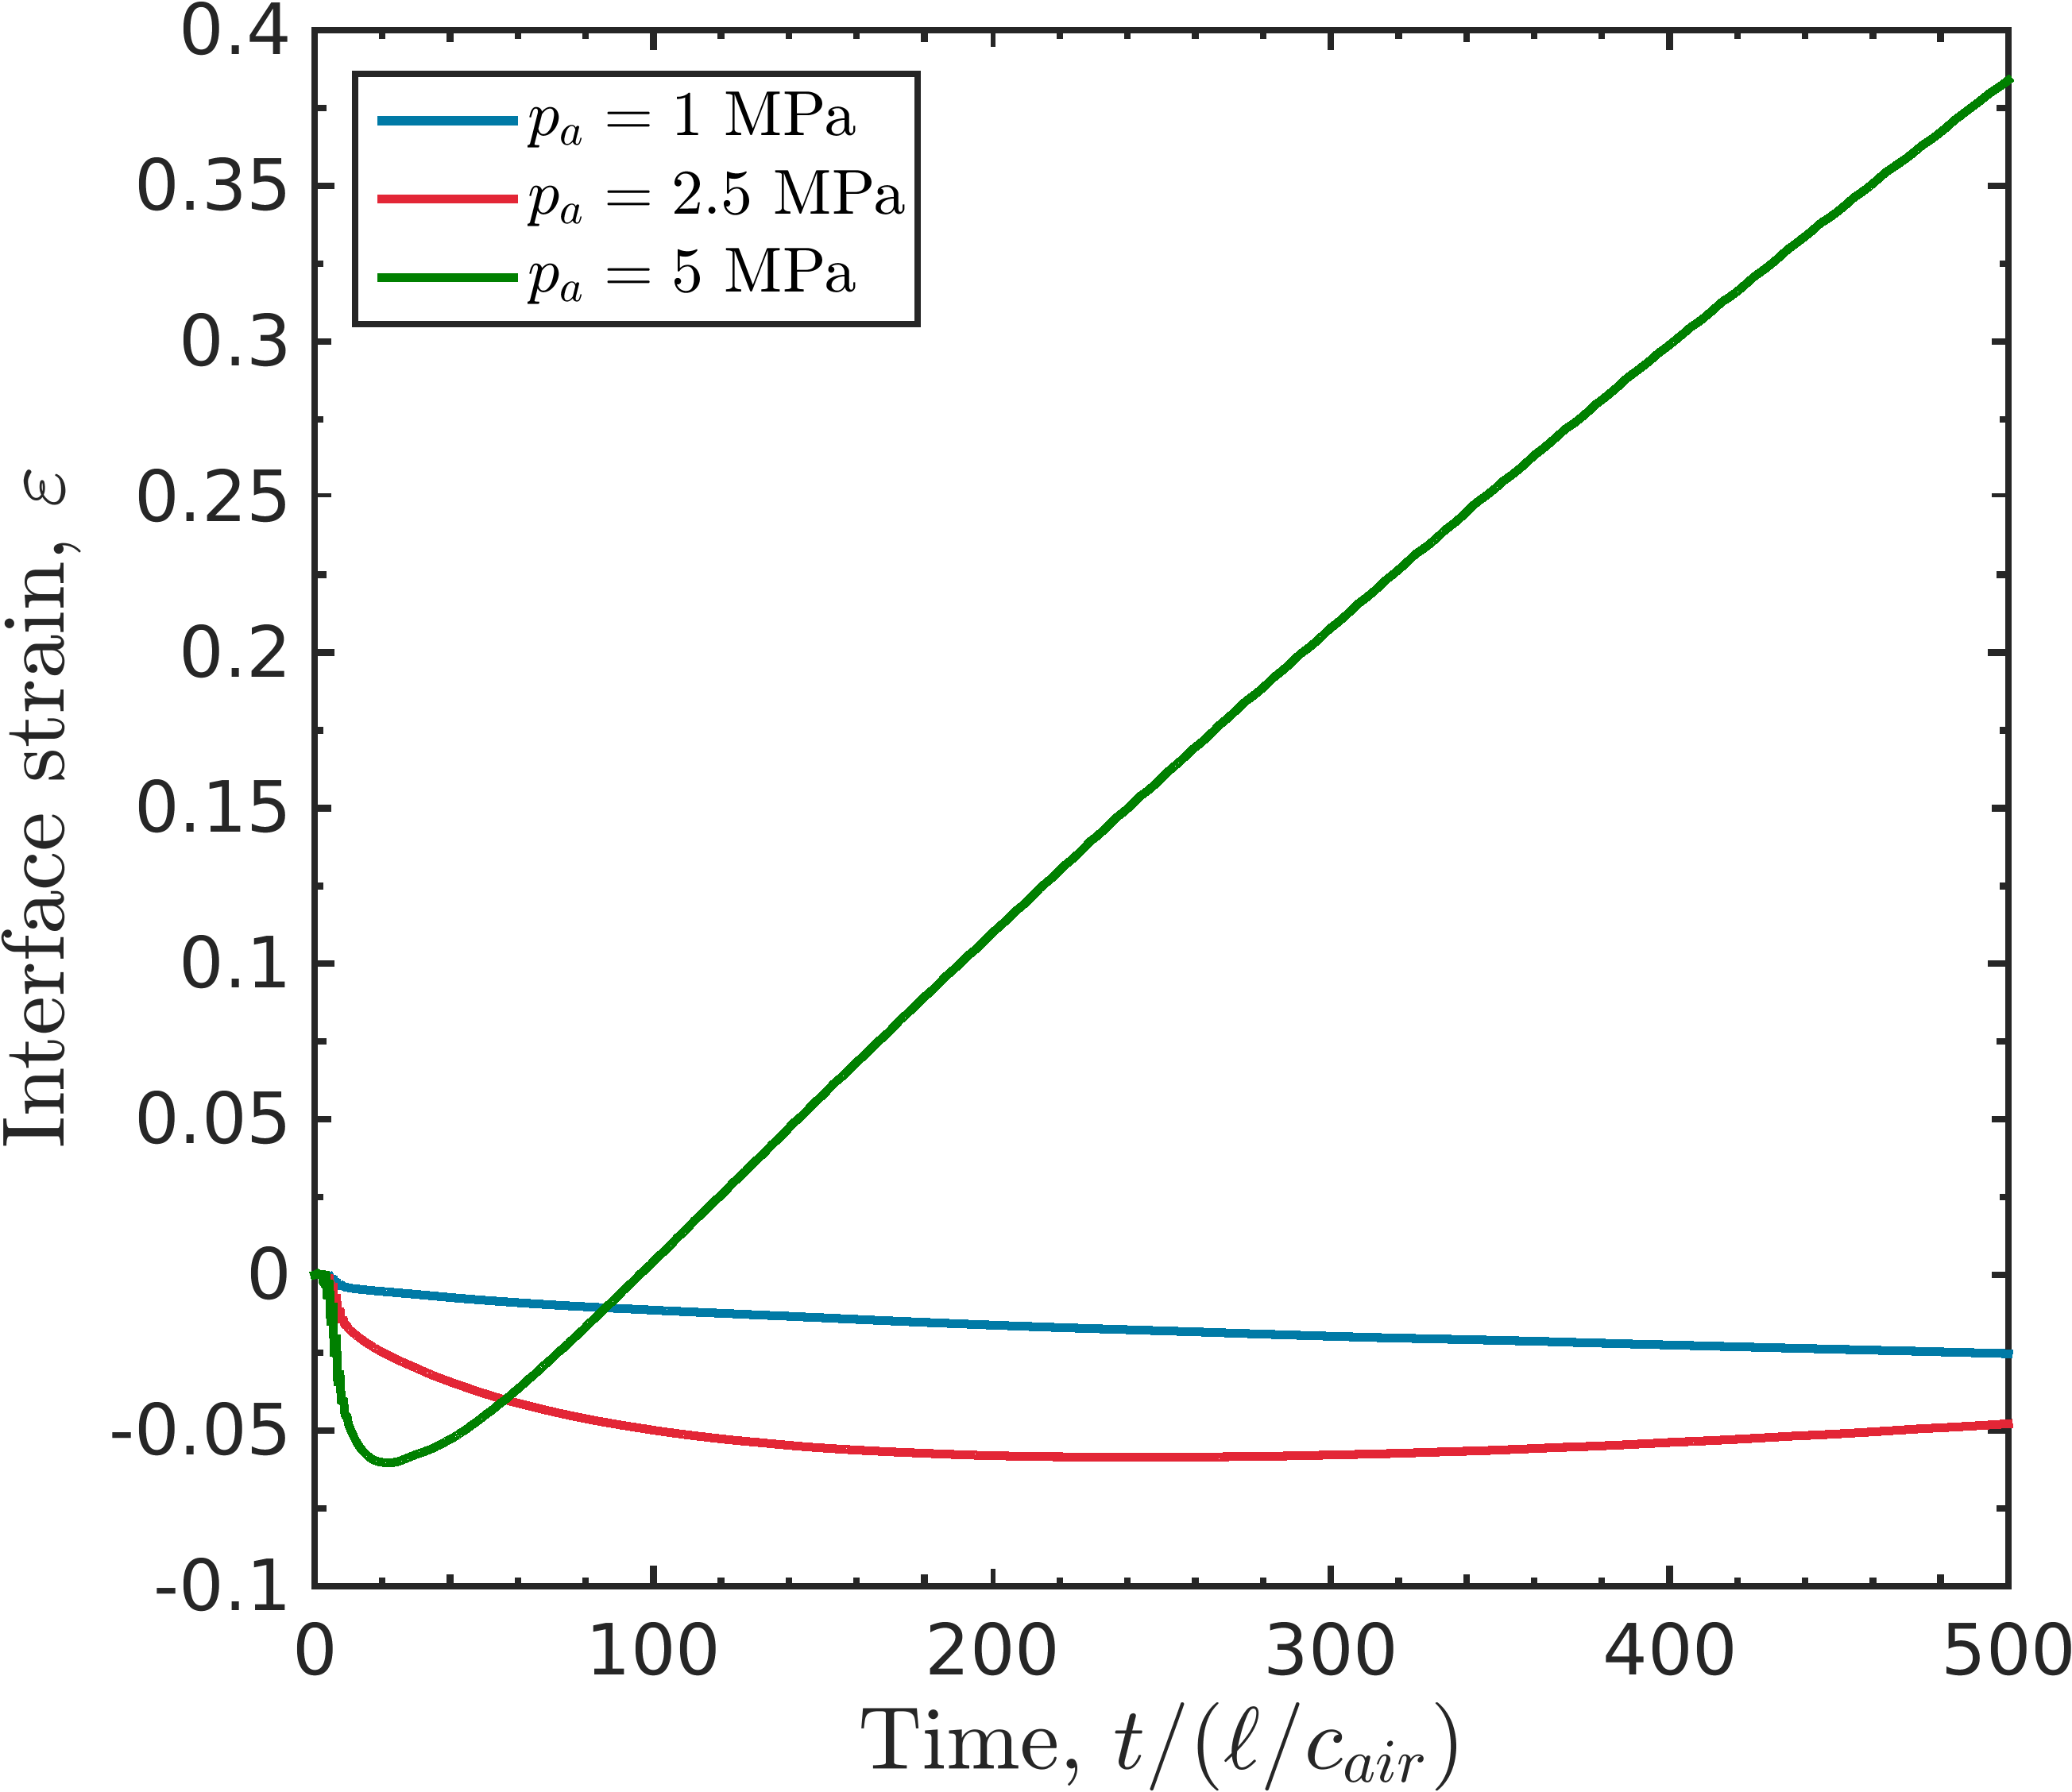
\includegraphics[width=\textwidth]{./figs/lung_figs/rmawave_1_A10,25,50_a30_strain_08-Mar-2017}
    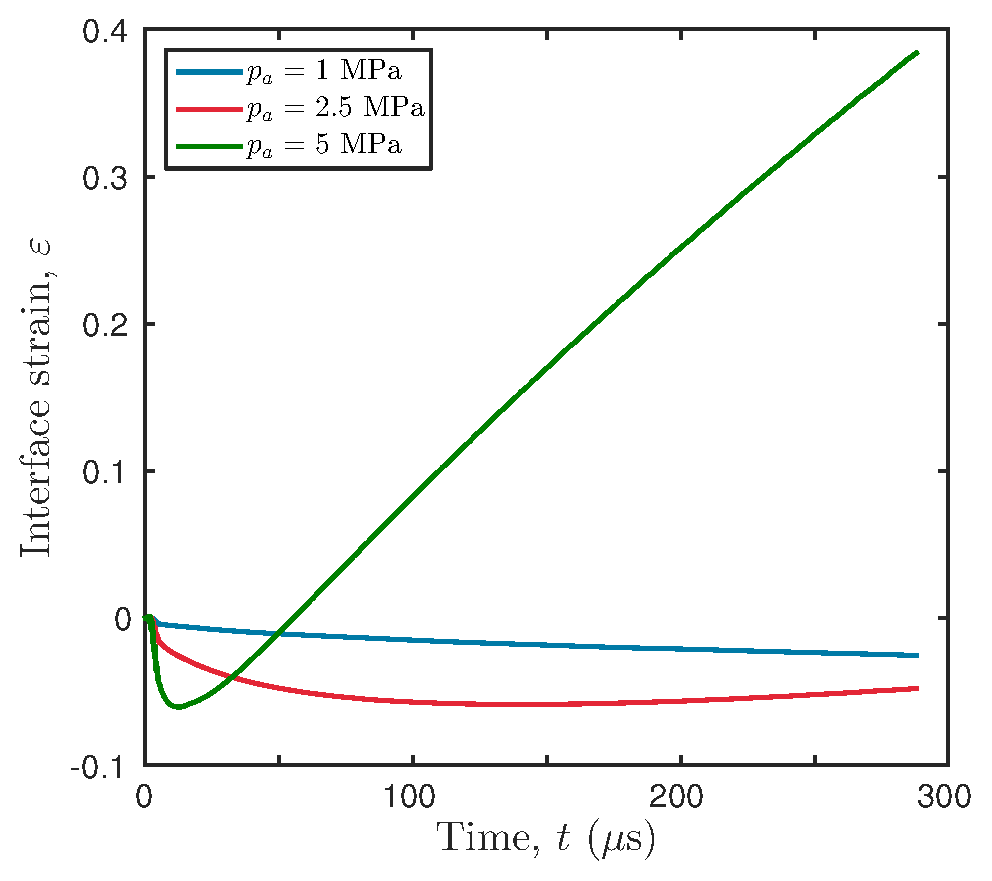
\includegraphics[width=\textwidth]{./figs/lung_figs/rmawave_1_A10,25,50_a30_strain_15-Jun-2017_dim}
    \caption{\label{fig:strain_multi-pa_a30} $a_0 = 0.30\ell$}
  \end{subfigure}
  % 
  \caption[Interfacial strain dependence on pressure amplitude
  ($p_a=1.0, 2.5, 5.0$ MPa)]%
  {Interfacial strain dependence on pressure amplitude
    ($p_a=1.0, 2.5, 5.0$ MPa). Each plot shows $\varepsilon$ for a
    different initial condition: $a_0=0.03\ell$
    \subref{fig:strain_multi-pa_a03}, $0.10\ell$
    \subref{fig:strain_multi-pa_a10}, and $0.30\ell$
    \subref{fig:strain_multi-pa_a30}.}
  \label{fig:pa_dependence_strain}
\end{figure}
% 
\begin{figure}
  \centering
  \begin{subfigure}[b]{0.49\textwidth}
    % 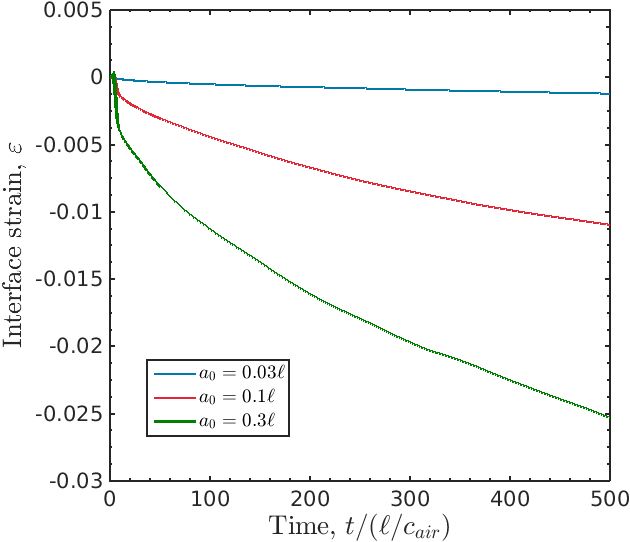
\includegraphics[width=\textwidth]{./figs/lung_figs/rmawave_1_A10_a03,10,30_strain_08-Mar-2017}
    \includegraphics[width=\textwidth]{./figs/lung_figs/rmawave_1_A10_a03,10,30_strain_15-Jun-2017_dim}
    \caption{\label{fig:strain_multi-a0-A10} $p_a = 1.0$ MPa}
  \end{subfigure}
  ~ 
  \begin{subfigure}[b]{0.49\textwidth}
    \includegraphics[width=\textwidth]{./figs/lung_figs/rmawave_1_A25_a03,10,30_strain_15-Jun-2017_dim}
    \caption{\label{fig:strain_multi-a0-A25} $p_a = 2.5$ MPa}
  \end{subfigure}
  ~
  \begin{subfigure}[b]{0.49\textwidth}
    % 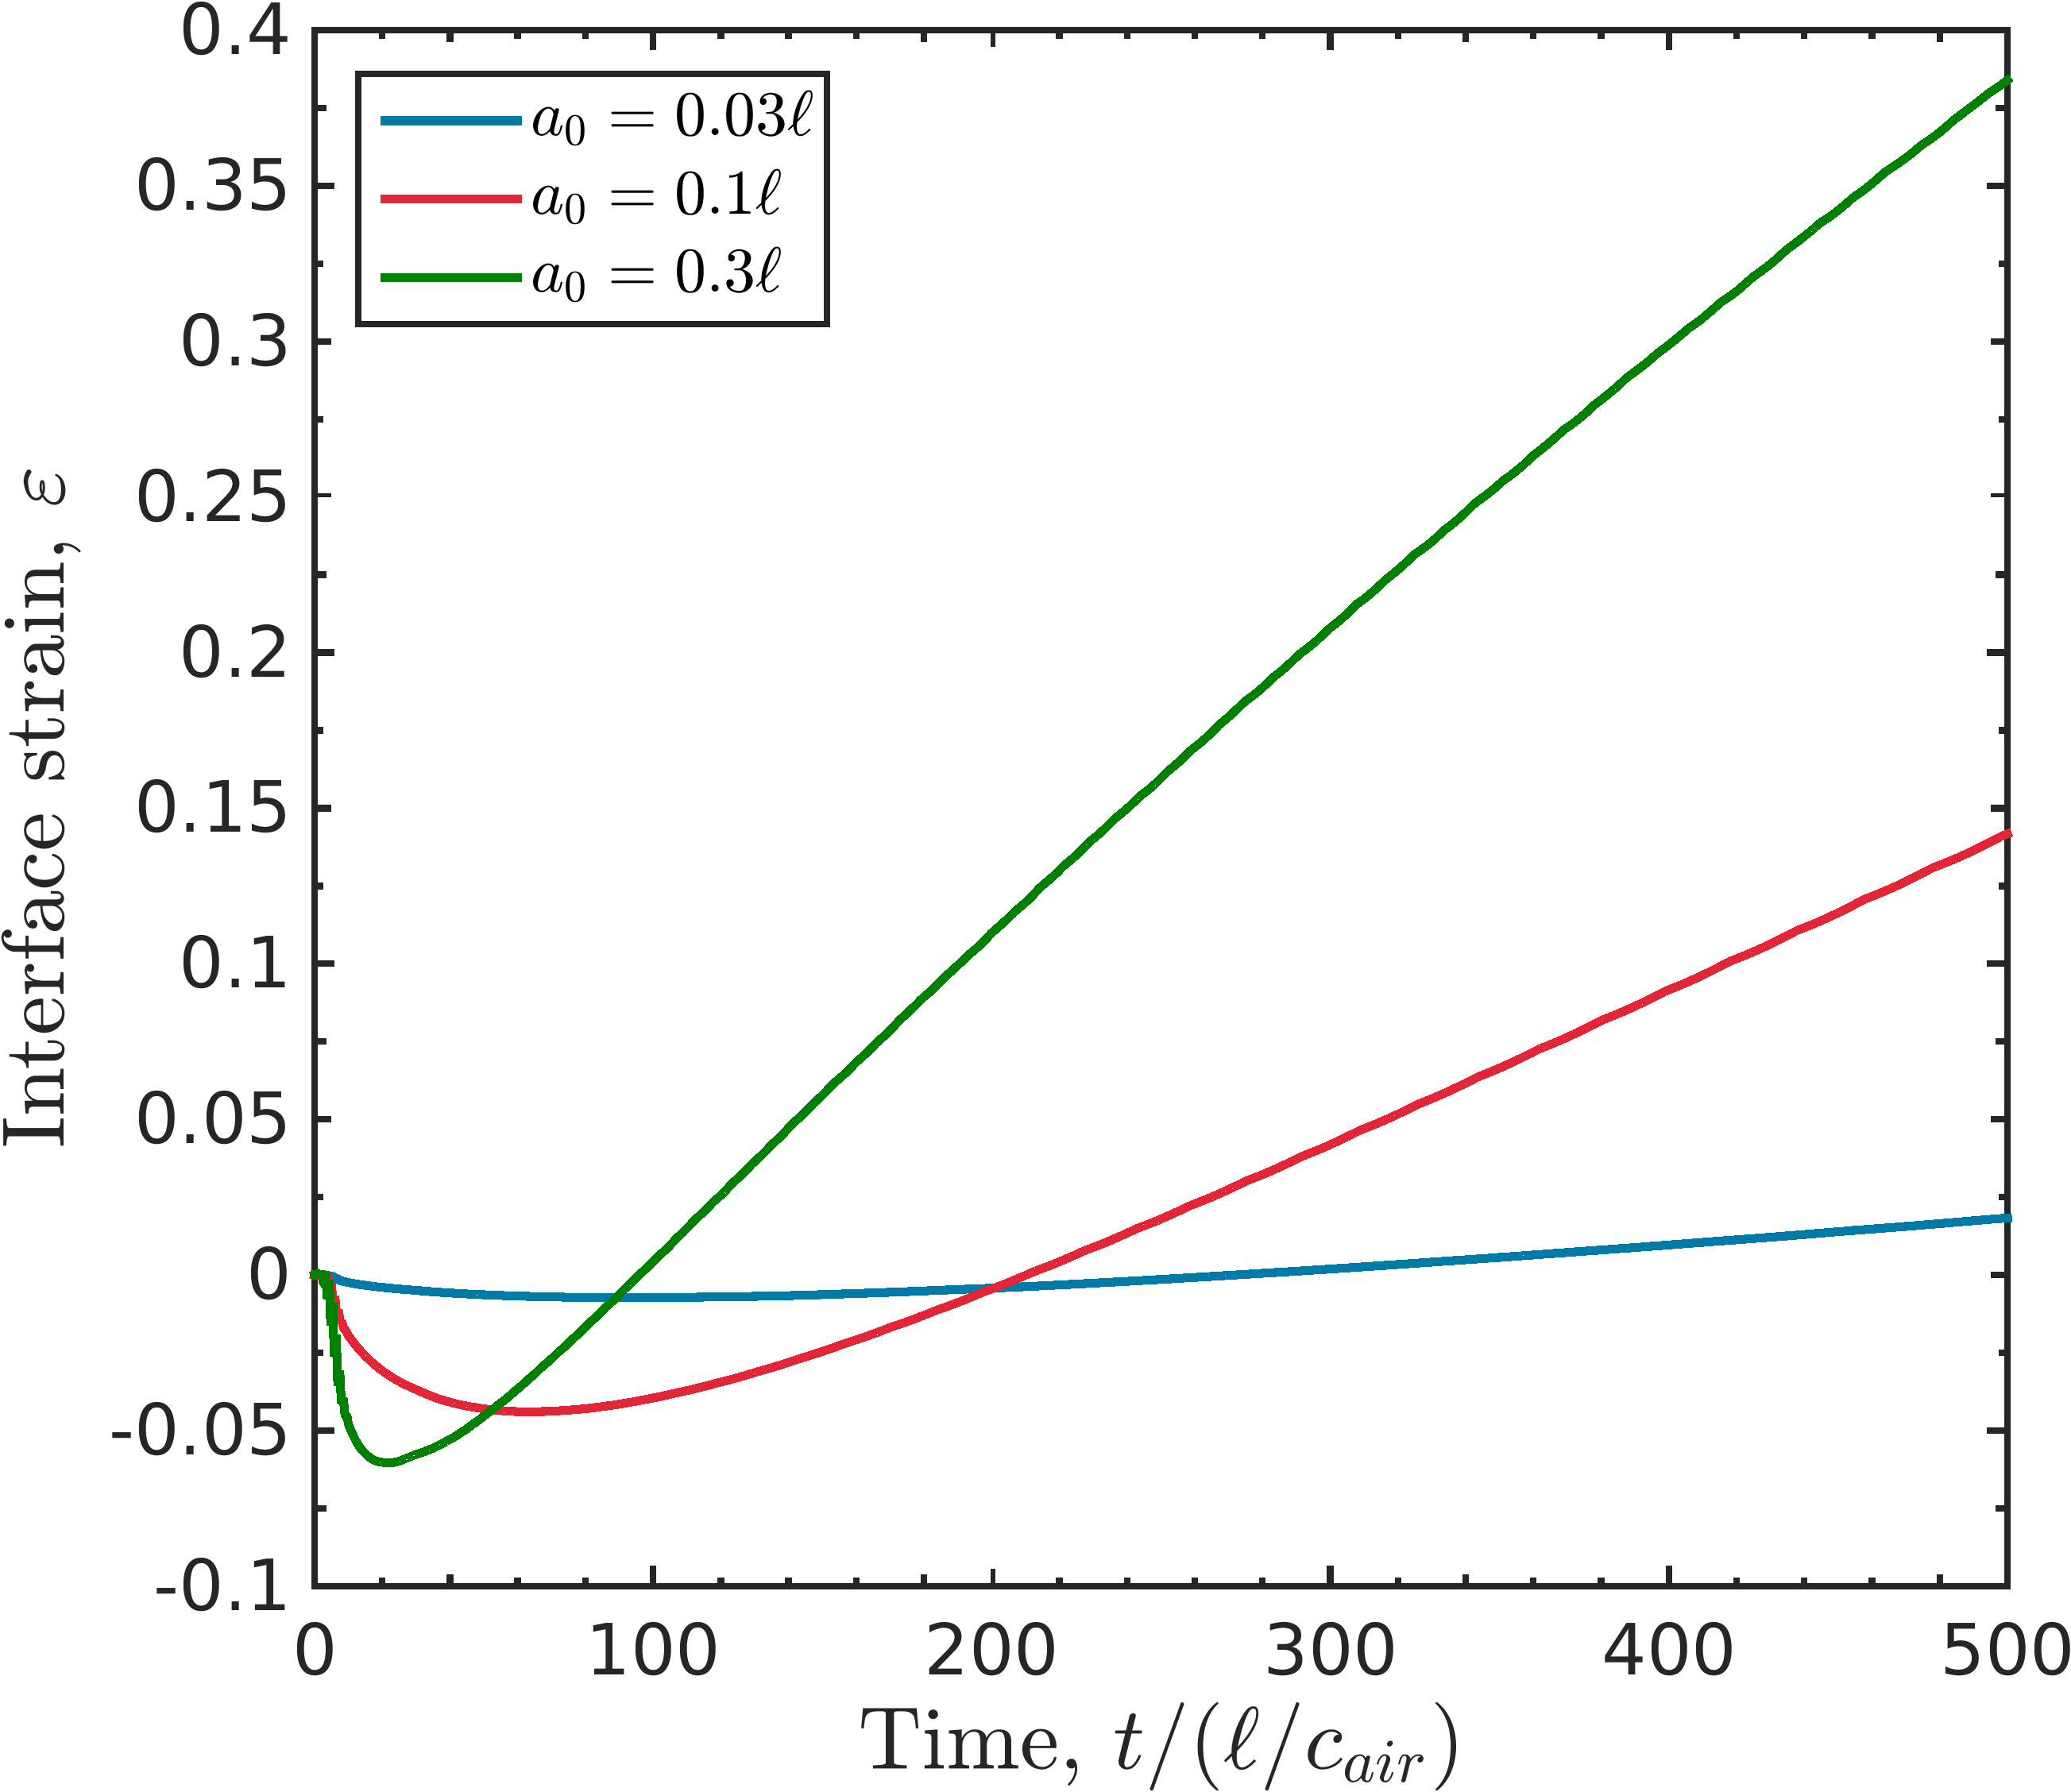
\includegraphics[width=\textwidth]{./figs/lung_figs/rmawave_1_A50_a03,10,30_strain_08-Mar-2017}
    \includegraphics[width=\textwidth]{./figs/lung_figs/rmawave_1_A50_a03,10,30_strain_15-Jun-2017_dim}
    \caption{\label{fig:strain_multi-a0-A50} $p_a = 5.0$ MPa}
  \end{subfigure}
  % 
  \caption[Interfacial strain dependence on initial perturbation
  amplitude ($a_0=0.03\ell,~0.10\ell,~0.30\ell$)]%
  {Interfacial strain dependence on initial perturbation amplitude
    ($a_0=0.03\ell,~0.10\ell,~0.30\ell$). Each plot shows $\varepsilon$
    for a different pulse amplitude: $p_a = 1.0 $ MPa
    \subref{fig:strain_multi-a0-A10}, $2.5$ MPa
    \subref{fig:strain_multi-a0-A25}, and $5.0$ MPa
    \subref{fig:strain_multi-a0-A50}.}
  \label{fig:a0_dependence_strain}
\end{figure}
% 
% 
\subsection{Viscous stress}
In further consideration of possible alveolar damage mechanisms, we
compute the inferred viscous shear stress field, based on the motion
of the inviscid flow, and the extract the maximum along the
interface. To illustrate the viscous stress around the interface,
color contours of the viscous stress fields are provided for the
$p_a = 5.0$ MPa wave in Figure \ref{fig:tauxy_snapshots} at
$t=2.9~\mu$s, approximately when the acoustic pulse and viscous stress
are at their maximum amplitudes. Subfigures
\subref{fig:tauxy_snapshot_A50_a03},
\subref{fig:tauxy_snapshot_A50_a10}, and
\subref{fig:tauxy_snapshot_A50_a30} again correspond to initial
perturbation amplitudes of $a_0 = 0.03\ell, 0.10\ell,$ and $0.30\ell$,
respectively. Black lines indicate isocontours of the volume fraction
of water $\alpha = 0.5$. Since the viscous shear stress is governed by
the velocity gradients in the fluid, which scale linearly with the
acoustic pressure gradients (See Equation
\ref{eq:acoustic_relations}), it is unsurprising that the greatest
viscous shear stress amplitudes occur during the wave-interface
interaction, and in particular close to the time when the maximum
pressure amplitude encounters the interface. The maximum viscous
stress is observed to occur in the lighter region of the interface, in
which the fluid is mostly air and the velocity gradients are
greatest. At this point in time, the fluid around the interface has
had little time to move as a result of the wave and consequently the
interface remains largely undeformed.

We extract the maximum viscous stress amplitudes from field
$\abs{\tau_{xy}}_{max}$, which were found to lie consistently along
the interface for all cases. To illustrate the dependence of
$\abs{\tau_{xy}}_{max}$ on the pulse amplitude $p_a$ and initial
perturbation amplitude $a_0$, Figure \ref{fig:pa_dependence_stress}
shows $\abs{\tau_{xy}}_{max}$ histories for variable $p_a = 1.0$
(blue), $2.5$ (red), and $5$ (green) MPa and constant initial
perturbation amplitude $a_0=0.03\ell$
\subref{fig:stress_multi-pa_a03}, $0.10\ell$
\subref{fig:stress_multi-pa_a10}, and $0.30\ell$
\subref{fig:stress_multi-pa_a30}, and Figure
\ref{fig:a0_dependence_stress} shows this data re-plotted for variable
$a_0 = 0.03\ell$ (blue), $0.10\ell$ (red), and $0.30\ell$ (green) and
constant wave amplitudes $p_a=1.0$ \subref{fig:stress_multi-a0-A10},
$2.5$ \subref{fig:stress_multi-a0-A25}, and $5.0$
\subref{fig:stress_multi-a0-A50} MPa. We highlight the fact that,
because we are intentionally only interested in the maximum
interfacial stress amplitude, the location along the interface at
which $\abs{\tau_{xy}}_{max}$ occurs changes in time, which is not
captured in the figures. For all waves and initial perturbation
conditions, $\abs{\tau_{xy}}_{max}$ oscillates with the wave during
the wave interaction, around a mean value which appears to rise and
fall with the acoustic intensity. We note that there is a component of
these oscillations that coincide with the fluctuations in the \ac{US}
pulse. These fluctuations occurs at approximately twice the pulse
frequency because we are considering the absolute value of the viscous
stress, which we expect to scale with the magnitude of the velocity
gradients and therefore the pulse amplitude (see the acoustic
relationships described in Chapter \ref{ch:usbe_lung}).

It is clear from both Figure \ref{fig:pa_dependence_stress} and
\ref{fig:a0_dependence_stress} that, on average, increasing the wave
amplitude increases the viscous stress amplitude at the interface as
expected (neglecting chronologically local oscillations). Regarding
the dependence of $\abs{\tau_{xy}}_{max}$ on $a_0$, we make two
observations. First, as $a_0$ increases, the chronologically local
mean value of $\abs{\tau_{xy}}_{max}$ also increases, though this is
slightly less obvious from the figures due to the varying degree of
oscillation between the curves. Second, based on differences between
Figures
\ref{fig:pa_dependence_stress}\subref{fig:stress_multi-a0-A10},
\subref{fig:stress_multi-a0-A25}, and
\subref{fig:stress_multi-a0-A50}, as $a_0$ increases, the oscillation
behavior changes. The overall magnitude of the osccillations in
$\abs{\tau_{xy}}_{max}$, relative to the chronologically local mean,
decreases. This is because as $a_0$ increases, a greater portion of
the reflected wave propagates in the transverse direction. These
transverse waves introduce additional oscillations in the shear stress
field, which are small when compared to those generated directly by
the incoming wave. These oscillations are identified according to
their timing and are most clearly explained with an example. Consider
$\abs{\tau_{xy}}_{max}$ for the $p_a=5$ MPa, $a_0=0.3\ell$ case, as
shown in Figure
\ref{fig:a0_dependence_strain}\subref{fig:strain_multi-a0-A50}. The
larger stress peaks occur approximately regularly during the wave
interaction every $0.3~\mu$s, and correspond to the interactions of
the peaks and troughs of the wave with the interface, as shown in
Figure \ref{fig:p0_ultrasound}. Shortly after each of these larger
peaks there is a slight drop in the peak stress. The time separating
the peak and drop is approximately $\ell/c\approx0.12~\mu$s,
indicating these fluctuations are a consequence of the transversely
reflected wave, which has the opposite sign of the incoming wave. We
note that axial reflections are small and do not return to the
interface until after the passage of the initial wave. After the
passage of the wave, the maximum shear stress drops to nearly zero in
all cases.

In consideration of \ac{DUS}-induced alveolar hemorrhage, we note that
for the parameters considered here the maximum viscous stress
amplitudes observed at the interface occur during the interaction with
the wave and ranged from $2$ to $61$ Pa. Even
the greatest observed stress is two orders of magnitude smaller the
$8$ kPa minimal stress failure threshold observed by \cite{West1991}
for disruption of alveolar epithelium. These stresses occur during
the wave-interface interaction, and quickly fall off thereafter, in
much less time than a typical period between pulses ($\sim 1$
ms). This suggests that viscous stresses are not likely to quickly
accumulate between pulses. A possible, exception to this could occur
if the velocity field were to change significantly, perhaps as a
result of accumulated vorticity from subsequent \ac{US} pulses. The
computational cost of testing this possibility numerically is not feasible under
the current framework, and as such is beyond the scope of this work.
% 
% 
\begin{figure}
  \captionsetup[subfigure]{labelformat=empty}
  \centering
  \begin{subfigure}[b]{0.3\textwidth}
    \begin{tikzpicture}%
      \node[anchor=south west,inner sep=0] (image) at (0,0) {
        \includegraphics[width=\textwidth]{./figs/lung_figs/rmawave_1_A50_a03_t005_tauxy_snapshots_dim_printable}
      };%
      \begin{scope}[x={(image.south east)},y={(image.north west)}]%
        \node[font=\small,right] at (0.2,0.9) {$\tau_{xy}$ (Pa)};%
        \node[font=\small,right] at (0.2,0.25) {$t = 2.9~\mu$s };%
      \end{scope}%  
    \end{tikzpicture}%
    \caption{\label{fig:tauxy_snapshot_A50_a03} $a_0 = 0.03\ell$}
  \end{subfigure}
  ~ 
  \begin{subfigure}[b]{0.3\textwidth}
    \begin{tikzpicture}%
      \node[anchor=south west,inner sep=0] (image) at (0,0) {
        \includegraphics[width=\textwidth]{./figs/lung_figs/rmawave_1_A50_a10_t005_tauxy_snapshots_dim_printable}
      };%
      \begin{scope}[x={(image.south east)},y={(image.north west)}]%
        \node[font=\small,right] at (0.2,0.9) {$\tau_{xy}$ (Pa)};%
        \node[font=\small,right] at (0.2,0.25) {$t = 2.9~\mu$s };%
      \end{scope}%  
    \end{tikzpicture}%
    \caption{\label{fig:tauxy_snapshot_A50_a10} $a_0 = 0.10\ell$}
  \end{subfigure}
  ~ 
  \begin{subfigure}[b]{0.3\textwidth}
    \begin{tikzpicture}%
      \node[anchor=south west,inner sep=0] (image) at (0,0) {
        \includegraphics[width=\textwidth]{./figs/lung_figs/rmawave_1_A50_a30_t500_tauxy_snapshots_dim_printable}
      };%
      \begin{scope}[x={(image.south east)},y={(image.north west)}]%
        \node[font=\small,right] at (0.2,0.9) {$\tau_{xy}$ (Pa)};%
        \node[font=\small,right] at (0.2,0.25) {$t = 2.9~\mu$s };%
      \end{scope}%  
    \end{tikzpicture}%
    \caption{\label{fig:tauxy_snapshot_A50_a30} $a_0 = 0.30\ell$}
  \end{subfigure}
  \caption[Evolution of the viscous stress field for the $p_a=5.0$ MPa
  wave]{Evolution of the viscous stress field for the $p_a=5.0$ MPa
    wave. Contour plots of the Newtonian viscous stress $\tau_{xy}$ in
    Pascals are shown for each initial perturbation amplitude, at
    $t=5$, near the point when the maximum stress occurs. In Figures
    \subref{fig:tauxy_snapshot_A50_a03},
    \subref{fig:tauxy_snapshot_A50_a10}, and
    \subref{fig:tauxy_snapshot_A50_a30} $a_0=0.03\ell,\, 0.10\ell,$ and
    $0.30\ell$ respectively.  }
  \label{fig:tauxy_snapshots}
  % 
\end{figure}

% \begin{comment}
%   \begin{figure}
%     \centering
%     \begin{subfigure}[b]{0.32\textwidth}
%       \begin{tikzpicture}%
%         \node[anchor=south west,inner sep=0] (image) at (0,0) {
%         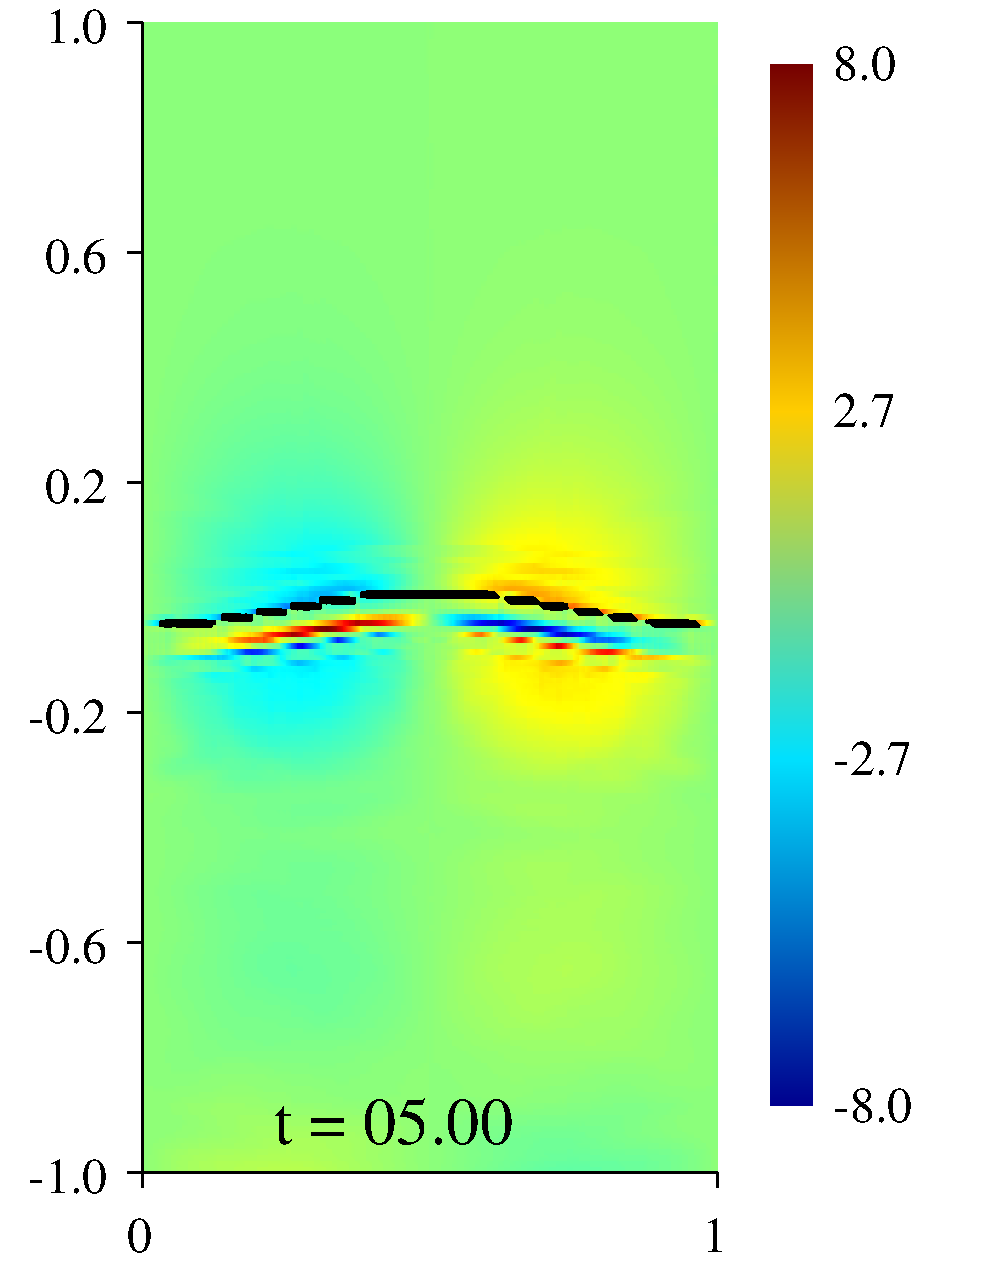
\includegraphics[width=\textwidth]{./figs/lung_figs/rmawave_1_A50_a03_t005_tauxy_snapshots}
%       };%
%         \begin{scope}[x={(image.south east)},y={(image.north
%           west)}]%
%           \node[font=\small,right] at (0.75,0.05) {$\tau_{xy}$
%           (Pa)};%
%         \end{scope}%
%       \end{tikzpicture}%
%       \caption{\label{fig:tauxy_snapshot_A50_a03} $a_0 = 0.03\ell$}
%     \end{subfigure}
%     ~
%     \begin{subfigure}[b]{0.32\textwidth}
%       \begin{tikzpicture}%
%         \node[anchor=south west,inner sep=0] (image) at (0,0) {
%         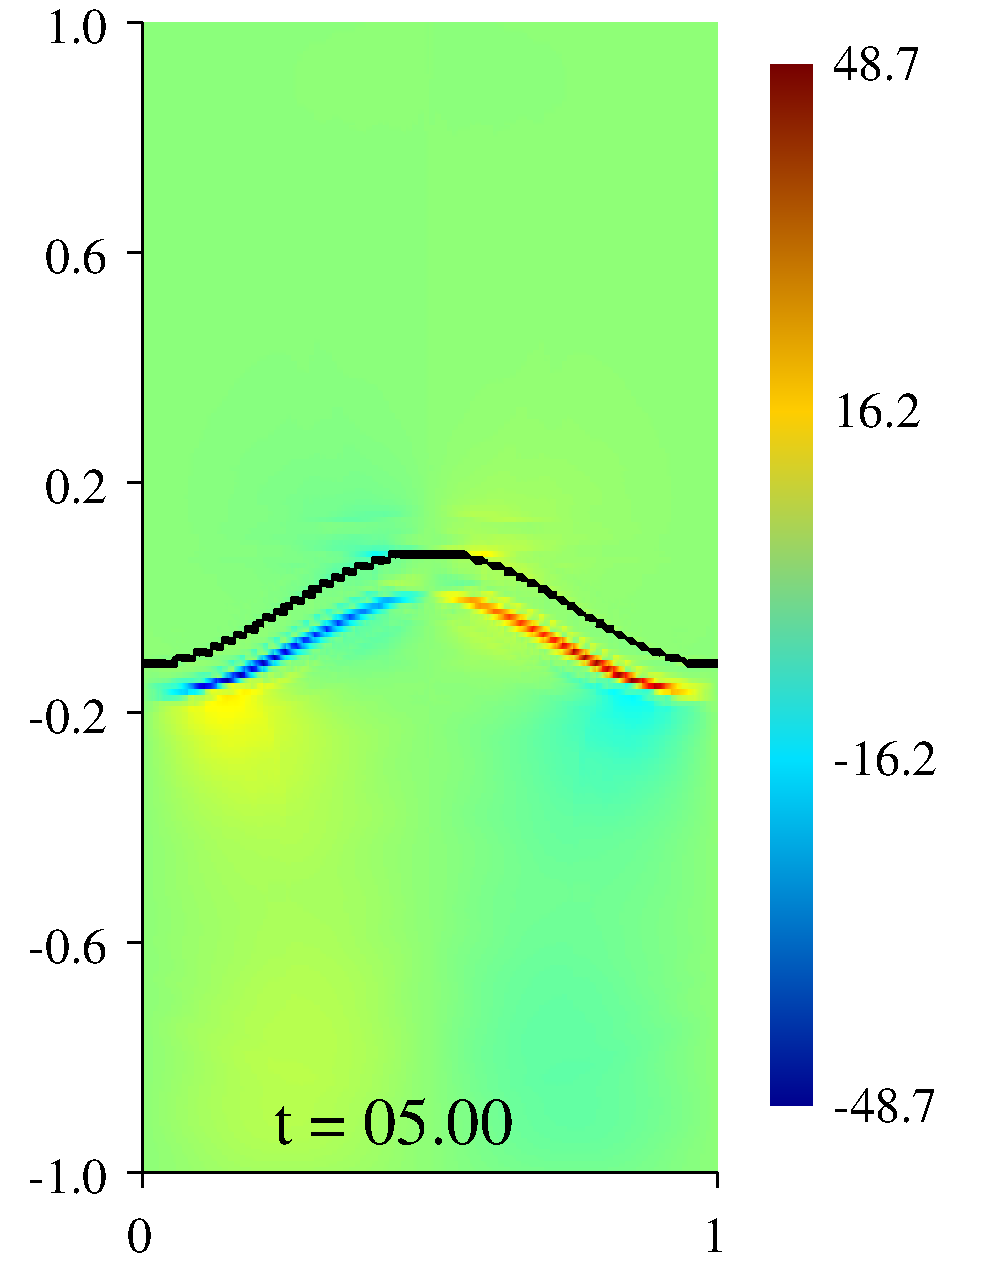
\includegraphics[width=\textwidth]{./figs/lung_figs/rmawave_1_A50_a10_t005_tauxy_snapshots}
%       };%
%         \begin{scope}[x={(image.south east)},y={(image.north
%           west)}]%
%           \node[font=\small,right] at (0.75,0.05) {$\tau_{xy}$
%           (Pa)};%
%         \end{scope}%
%       \end{tikzpicture}%
%       \caption{\label{fig:tauxy_snapshot_A50_a10} $a_0 = 0.10\ell$}
%     \end{subfigure}
%     ~
%     \begin{subfigure}[b]{0.32\textwidth}
%       \begin{tikzpicture}%
%         \node[anchor=south west,inner sep=0] (image) at (0,0) {
%         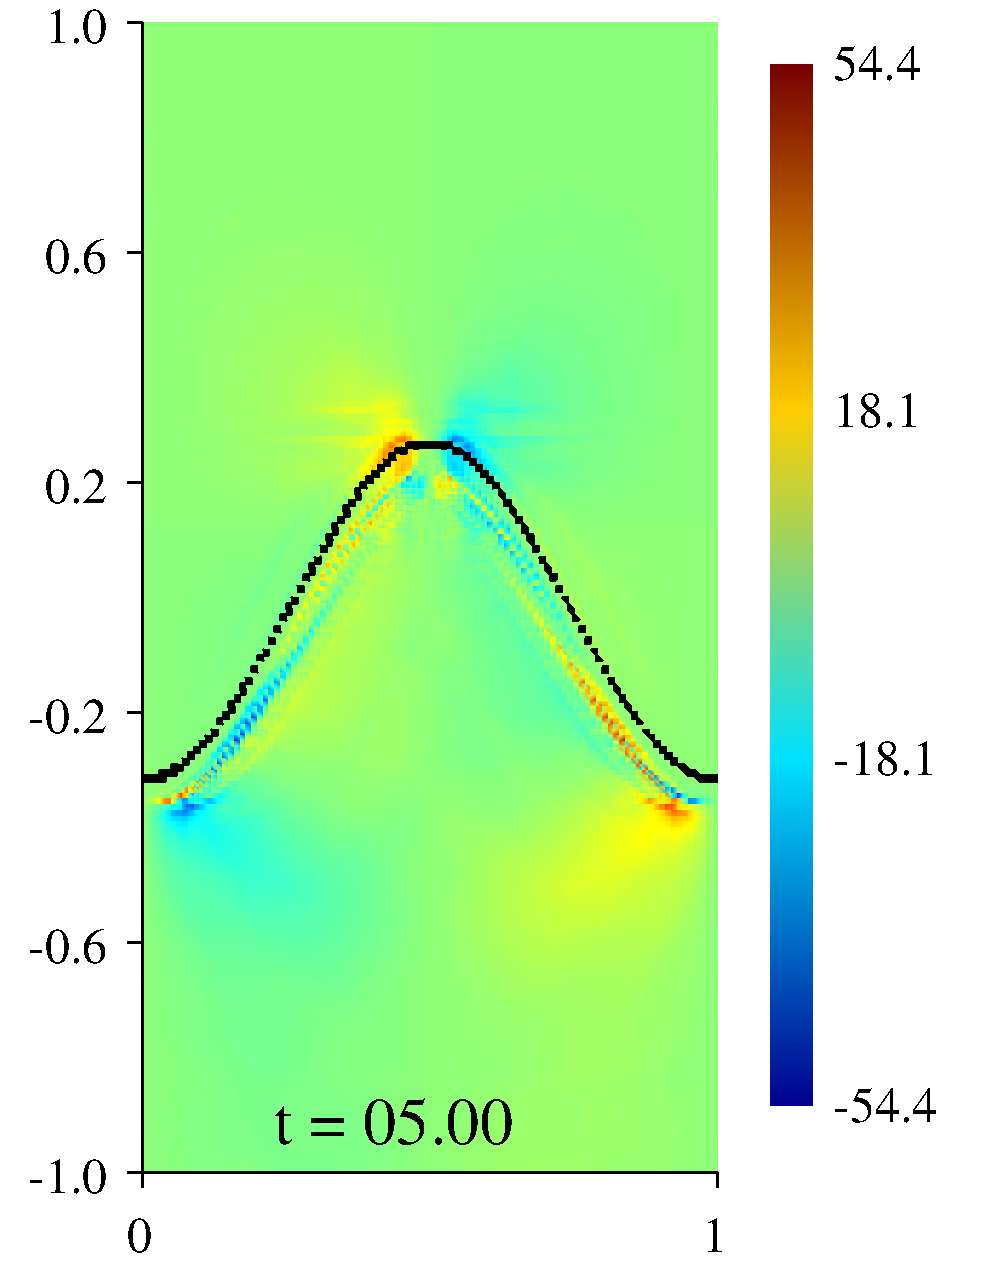
\includegraphics[width=\textwidth]{./figs/lung_figs/rmawave_1_A50_a30_t500_tauxy_snapshots}
%       };%
%         \begin{scope}[x={(image.south east)},y={(image.north
%           west)}]%
%           \node[font=\small,right] at (0.75,0.05) {$\tau_{xy}$
%           (Pa)};%
%         \end{scope}%
%       \end{tikzpicture}%
%       \caption{\label{fig:tauxy_snapshot_A50_a30} $a_0 = 0.30\ell$}
%     \end{subfigure}
%     %     
%     \caption{Contour plots of the Newtonian viscous stress
%     $\tau_{xy}$ in Pascals are shown for each initial perturbation
%     amplitude for the $p_a=5.0$ MPa pulse at $t=5$, near the point
%     when the maximum stress occurs. In Figures
%     \subref{fig:tauxy_snapshot_A50_a03},
%     \subref{fig:tauxy_snapshot_A50_a10}, and
%     \subref{fig:tauxy_snapshot_A50_a30} $a_0=0.03\ell,\, 0.10\ell,$
%     and $0.30\ell$ respectively.  }
%     \label{fig:tauxy_snapshots}
%   \end{figure}
% \end{comment}
% 
\begin{figure}
  \centering
  \begin{subfigure}[b]{0.49\textwidth}
    % 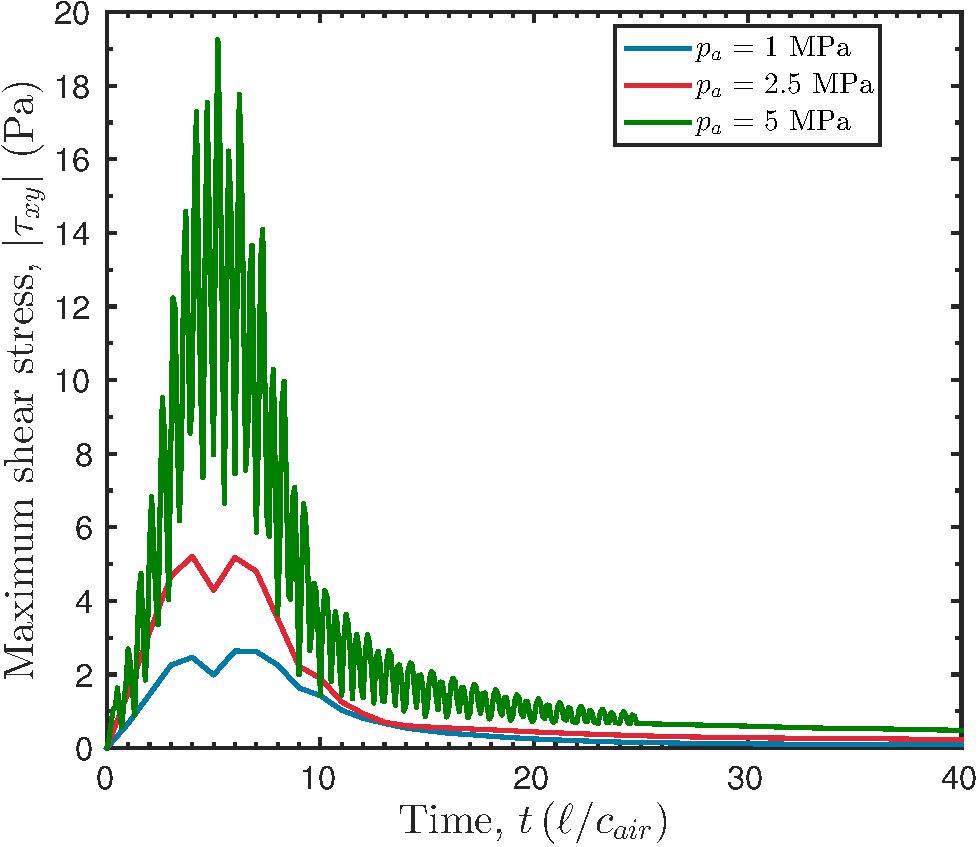
\includegraphics[width=\textwidth]{./figs/lung_figs/rmawave_1_A10,25,50_a3_tauxy_27-Feb-2017}
    \includegraphics[width=\textwidth]{./figs/lung_figs/rmawave_1_A10,25,50_a03_tauxy_07-Mar-2017_dim}
    \caption{\label{fig:stress_multi-pa_a03} $a_0 = 0.03\ell$}
  \end{subfigure}
  ~ 
  \begin{subfigure}[b]{0.49\textwidth}
    % 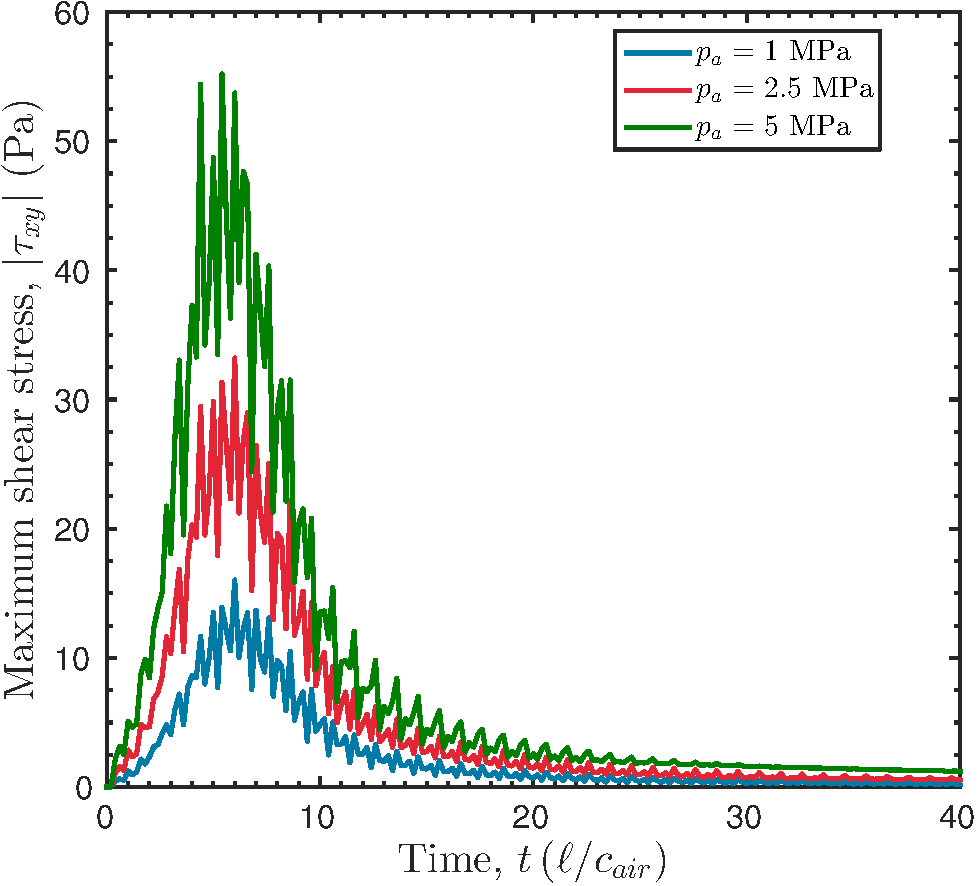
\includegraphics[width=\textwidth]{./figs/lung_figs/rmawave_1_A10,25,50_a10_tauxy_27-Feb-2017}
    \includegraphics[width=\textwidth]{./figs/lung_figs/rmawave_1_A10,25,50_a10_tauxy_07-Mar-2017_dim}
    \caption{\label{fig:stress_multi-pa_a10} $a_0 = 0.10\ell$}
  \end{subfigure}
  ~ 
  \begin{subfigure}[b]{0.49\textwidth}
    % 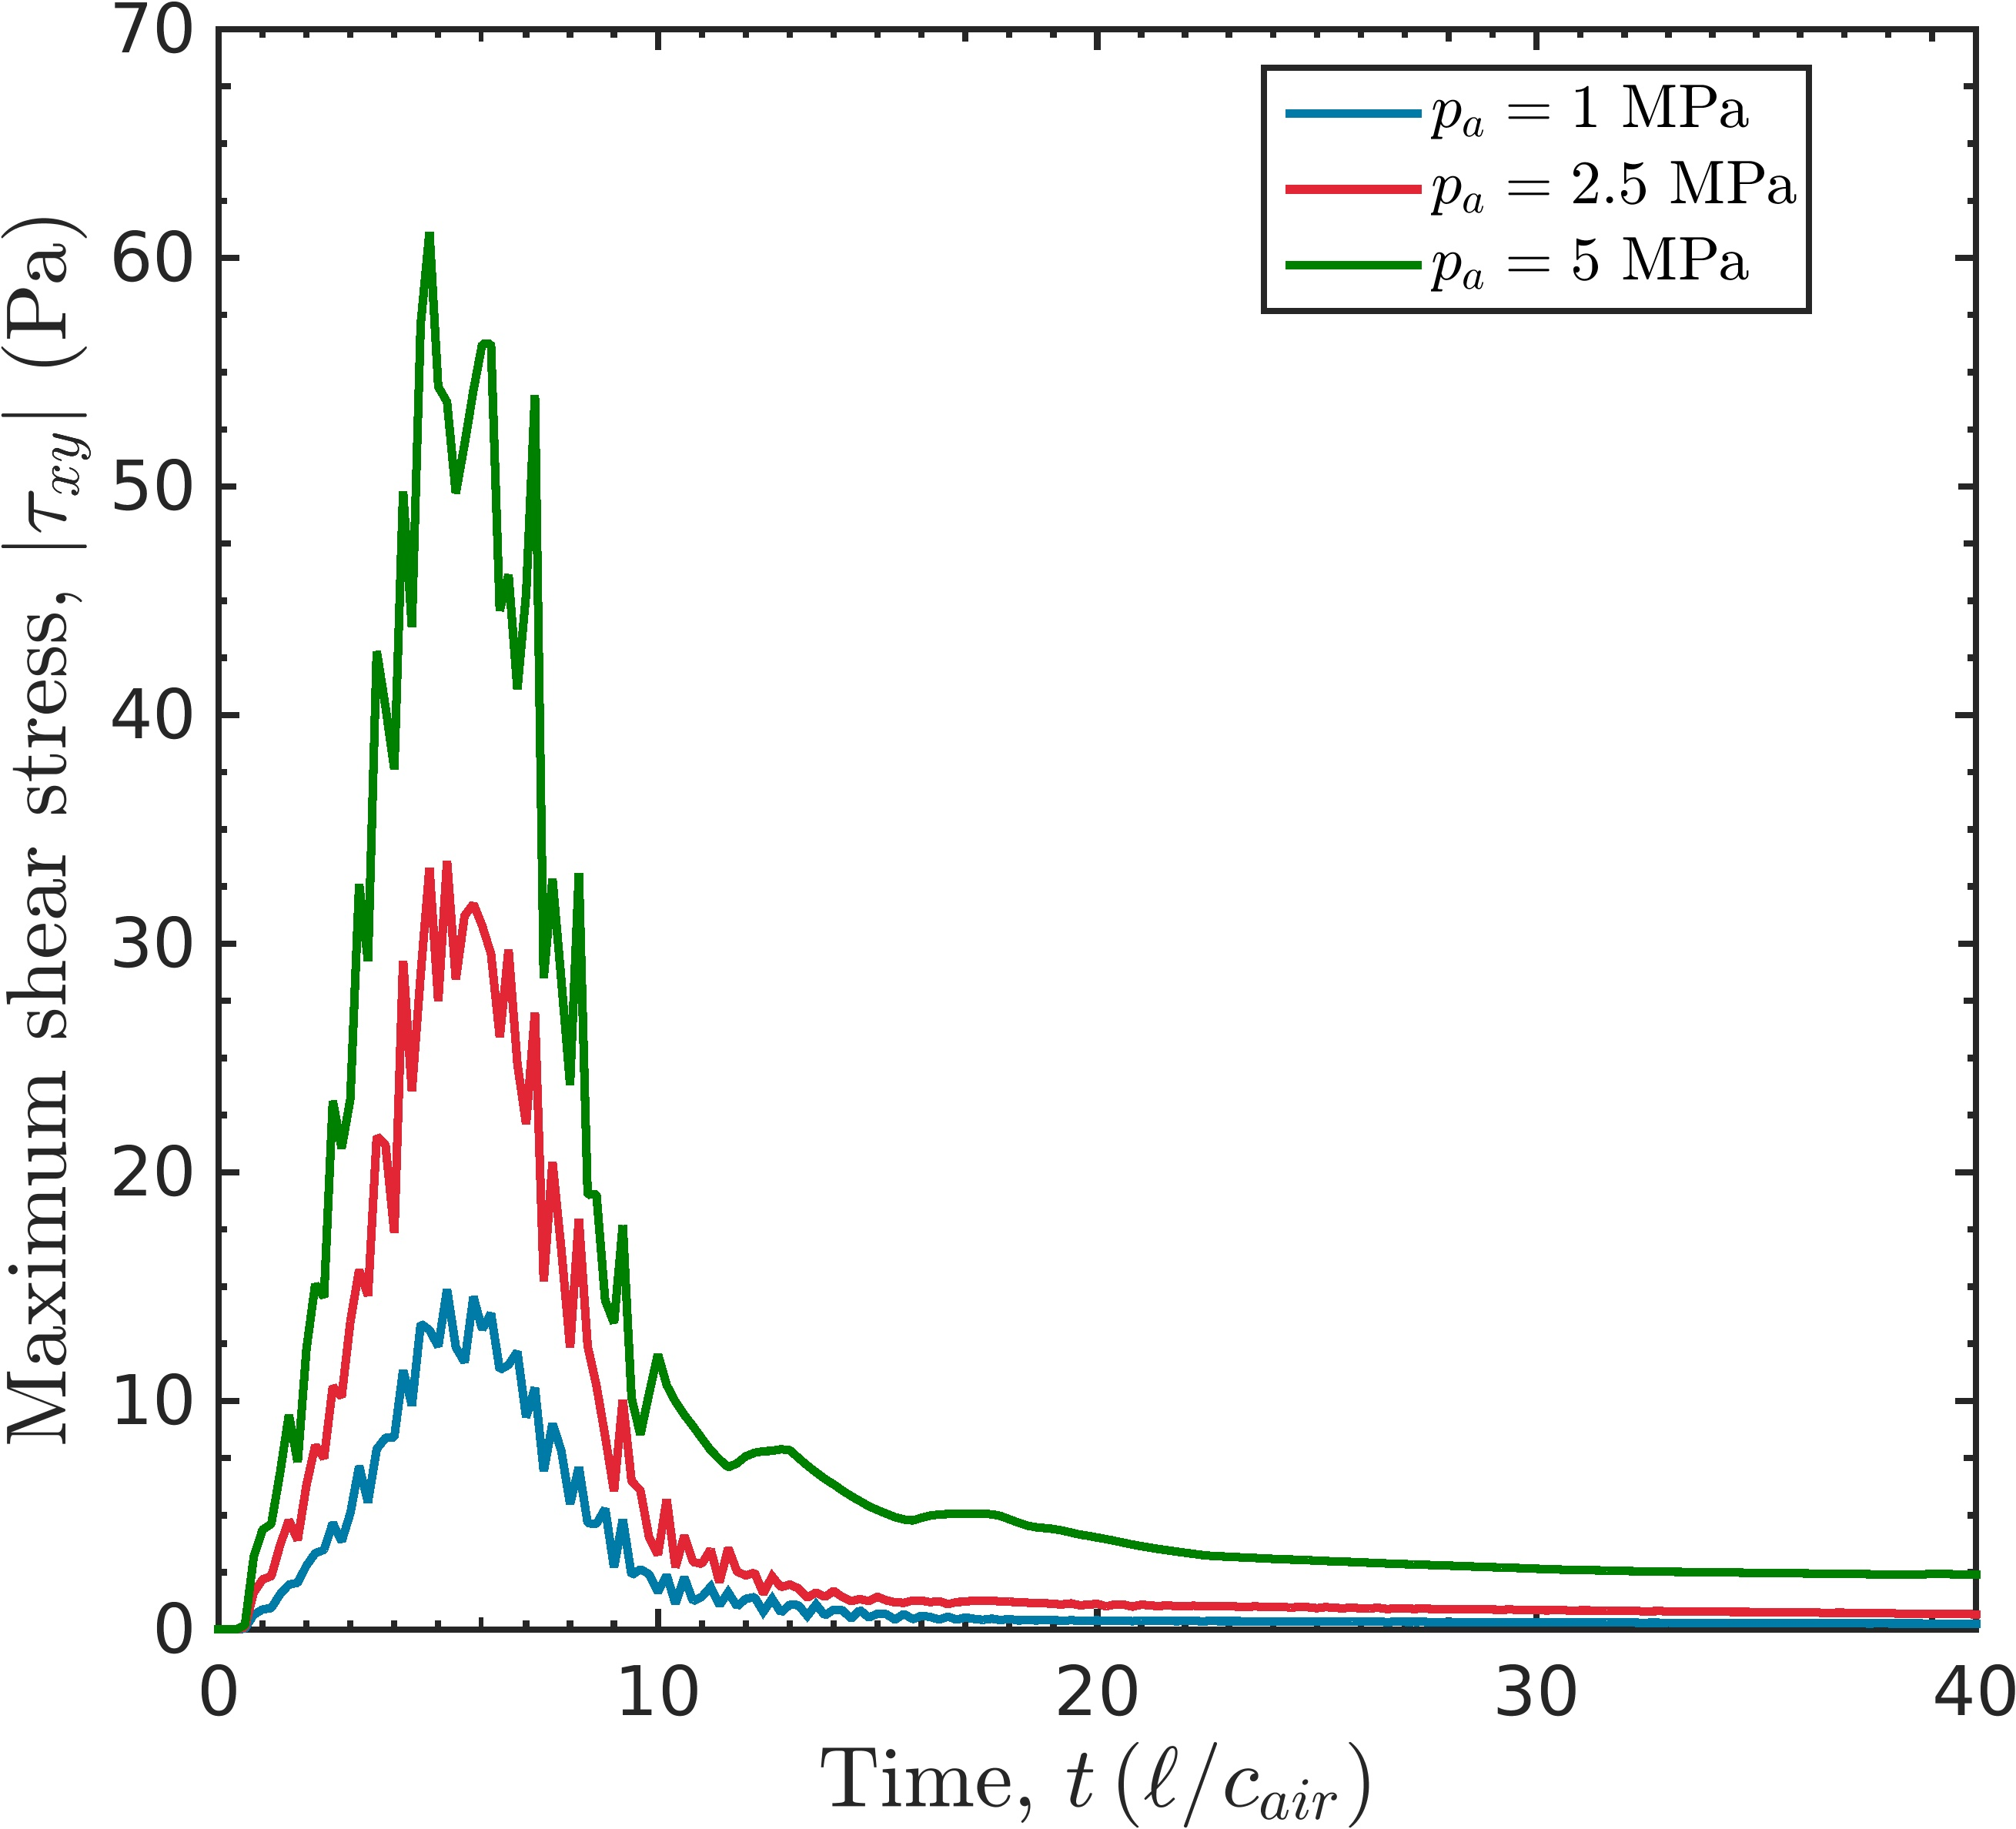
\includegraphics[width=\textwidth]{./figs/lung_figs/rmawave_1_A10,25,50_a30_tauxy_27-Feb-2017}
    \includegraphics[width=\textwidth]{./figs/lung_figs/rmawave_1_A10,25,50_a30_tauxy_07-Mar-2017_dim}
    \caption{\label{fig:stress_multi-pa_a30} $a_0 = 0.30\ell$}
  \end{subfigure}
  % 
  \caption[Interfacial viscous stress dependence on pressure
  amplitude ($p_a=1.0, 2.5, 5.0$ MPa)]{Interfacial viscous stress
    dependence on on pressure amplitude ($p_a=1.0, 2.5, 5.0$ MPa). Each
    plot shows $\left|\tau_{xy}\right|_{max}$ for a different initial
    condition: $a_0=0.03\ell$ \subref{fig:stress_multi-pa_a03},
    $0.10\ell$ \subref{fig:stress_multi-pa_a10}, and $0.30\ell$
    \subref{fig:stress_multi-pa_a30}.}
  \label{fig:pa_dependence_stress}
\end{figure}
% 
\begin{figure}
  \centering
  \begin{subfigure}[b]{0.49\textwidth}
    \includegraphics[width=\textwidth]{./figs/lung_figs/rmawave_1_A10_a3,10,30_tauxy_27-Feb-2017_dim}
    \caption{\label{fig:stress_multi-a0-A10} $p_a = 1.0$ MPa}
  \end{subfigure}
  ~
  \begin{subfigure}[b]{0.49\textwidth}
    \includegraphics[width=\textwidth]{./figs/lung_figs/rmawave_1_A25_a3,10,30_tauxy_27-Feb-2017_dim}
    \caption{\label{fig:stress_multi-a0-A25} $p_a = 2.5$ MPa}
  \end{subfigure}
  ~ 
  \begin{subfigure}[b]{0.49\textwidth}
    \includegraphics[width=\textwidth]{./figs/lung_figs/rmawave_1_A50_a3,10,30_tauxy_27-Feb-2017_dim}
    \caption{\label{fig:stress_multi-a0-A50} $p_a = 5.0$ MPa}
  \end{subfigure}
  % 
  \caption[Interfacial viscous stress dependence on initial
  perturbation amplitude amplitude
  ($a_0=0.03\ell, 0.10\ell, 0.30\ell$)]{Interfacial viscous stress
    dependence on initial perturbation amplitude amplitude
    ($a_0=0.03\ell, 0.10\ell, 0.30\ell$). Each plot shows
    $\left|\tau_{xy}\right|_{max}$ for a different pulse amplitude:
    $p_a = 1.0$\subref{fig:stress_multi-a0-A10},
    $2.5$\subref{fig:stress_multi-a0-A25}, and
    $5.0$\subref{fig:stress_multi-a0-A50} MPa.}
  \label{fig:a0_dependence_stress}
\end{figure}
% 
% 
% 
% 
% 
% 
\subsection{Ultrasound-induced vorticity dynamics and interface growth}
\label{subsec:vorticity_experiments}
Having examined the stresses and strains associated with liquid-gas
interfaces driven by \ac{US} pulse waves, within the regime relevant
to clinical \ac{DUS}, we now hypothesize that the observed deformation
is driven by baroclinic vorticity deposited at the liquid-gas
interface by the \ac{US} pulse. As there is still a highly nonlinear
density gradient across the interface, misaligned with strong
ultrasonic pressure gradients, the potential for meaningful baroclinic
vorticity deposition, and consequently persistent of the system,
exists. As we demonstrated that this was possible for a trapezoidal
acoustic wave in Chapter \ref{ch:usbe_lung}, we consider a second set
of experiments, designed to test if this holds true for the ultrasound
pulse. We will compare the interface and vorticity dynamics of an
ultrasound driven pulse, with those of the trapezoidal pulse of the
Chapter \ref{ch:usbe_lung}. The $1.0$ to $5.0$ MPa pulses used earlier
in this chapter drive the system too slowly for the interface growth
to reach its late-time behavior within a computationally feasible
period. Additionally, we aim to compare to our previous results and as
such we choose our acoustic pulse parameters and initial interface
perturbation amplitude to match that of our baseline trapezoidal wave
case Chapter \ref{ch:usbe_lung}: $a_0=0.03\ell$; $p_a = 10$ MPa;
$L=45\ell$. To further facilitate comparison of this experiment to
those of the previous chapter, all results presented here will be
non-dimensionalized by $\ell$ and $c_{water}$ unless otherwise
indicated.

To illustrate the vorticity during and after the passage of the wave,
Figure \ref{fig:Vorticity_circ_us}\subref{fig:us_vorticity_snapshot}
shows vorticity contours for the $p_a = 10$ MPa pulse wave case, at
$t/(\ell/c) = 4.75$ and $90$ (or $t = 0.6 $ and $12~\mu$s). It can be
clearly seen that vorticity is deposited along the interface by the
ultrasound wave, and remains after its passing. In consideration of a
quantitative, cumulative measure of vorticity deposited by the
ultrasound wave we integrate the vorticity at over the right-half
domain for each point in time to obtain the circulation,
$\Gamma(t)$. Figure
\ref{fig:Vorticity_circ_us}\subref{fig:us10_circulation_history} plots
the right-half domain circulation history during the wave interaction
and shortly thereafter. The end of the interaction between the
incident wave and the interface is indicated as a black, dashed
vertical line $t/(\ell/c) = 47.5$. It can be seen that the wave
deposits circulation, which remains approximately constant after its
passage. The circulation left at the end of the wave is approximately
$3 \times 10^{-4}$, which is roughly $1/5$ that left by the $p_a = 10$
MPa trapezoidal wave in Chapter \ref{ch:usbe_lung}. We note that
unlike the trapezoidal wave, which consists entirely of positive
pressure, the \ac{US} pulse consists of cyclic positive and negative
pressure, such that each subsequent cycle is expected to deposit
vorticity of sign opposite that of the previous cycle, since a phase
inversion of the interface perturbation was not observed during the
wave-interface interaction. Hence it is perhaps unsurprising that less
circulation is deposited by the ultrasound pulse than by the
trapezoidal wave of equivalent maximum amplitude. As in the previous
chapter, the circulation in the left-half domain is equal and opposite,
such that the total circulation is zero. Similar circulation histories
for the $p_a = 1.0, 2.5,$ and $5.0$ MPa waves, used in the earlier
stress and strain calculations, are provided in Appendix
\ref{sec:us_pulse_circulation}, and reveal that similar to the
$p_a = 10$ MPa case, circulation remains after the passage of the
wave. Appendix \ref{sec:us_pulse_circulation} also explores the
dependence of that circulation on $a_0$ and $p_a$ for the case of the
ultrasound pulse.%
\begin{figure}
  \centering
  \vfill
  \begin{subfigure}[t]{0.6\textwidth}
    \centering
    \begin{tikzpicture}
      \node[anchor=south west,inner sep=0] (image) at (0,0) {%
        \includegraphics[height=0.49\textwidth]{./figs/lung_figs/vorticity_t1_rmawave_1_10000000,0_0,03_45,0_0,0_1,0_1,0_1000_100_01-Aug-2017}
        \includegraphics[height=0.49\textwidth]{./figs/lung_figs/vorticity_t20_rmawave_1_10000000,0_0,03_45,0_0,0_1,0_1,0_1000_100_nocb}
      };%
      \begin{scope}[x={(image.south east)},y={(image.north west)}]%
        \node[font=\small,align=left,right] at (0.1,0.9){{$t=4.75$}};%
        \node[font=\small,align=left,right] at (0.4,0.9){{$(a)$}};%
        \node[font=\small,align=left,right] at (0.6,0.9){{$t=95$}};%
      \end{scope}%
    \end{tikzpicture}
    \phantomcaption%{Vorticity Contours}
    \label{fig:us_vorticity_snapshot}
  \end{subfigure}
  \hfill
  ~
  \begin{subfigure}[t]{0.35\textwidth}
    \begin{tikzpicture}
      \node[anchor=south west,inner sep=0] (image) at (0,0) {%
        \includegraphics[width=\textwidth]{./slides/figs/trapz_us_circ_comparison_A10_waveend_t0_t60_asa_01-Aug-2017}
      };%
      \begin{scope}[x={(image.south east)},y={(image.north west)}]%
        \node[font=\small,align=left,right] at
        (0.85,0.85){{(b)}};%
      \end{scope}%
    \end{tikzpicture}
    \phantomcaption%{Circulation, $\Gamma = \int_{A_R} \omega dA$}
    \label{fig:us10_circulation_history}
  \end{subfigure}
  \caption[Vorticity and circulation histories for the $p_a=10$ MPa
  ultrasound pulse.]{Vorticity and circulation histories for the
    $p_a=10$ MPa ultrasound pulse. \subref{fig:us_vorticity_snapshot}
    Vorticity contours during the wave interaction, at
    $t/(\ell/c)=4.75$ and after its passage at
    $t/(\ell/c)=90$. \subref{fig:us10_circulation_history} The
    dimensionless circulation history. The passage of the wave at
    $t/(\ell/c)=47.5$ is indicated as a black, dashed vertical line.}
  \label{fig:Vorticity_circ_us}
\end{figure}%

To compare the late time growth of the perturbation amplitude driven
by the ultrasound wave, with that driven by the trapezoidal wave,
Figure \ref{fig:us10_interface_growth} displays the perturbation
amplitude history $a(t)/a_0$ on a log-log scale. For
$t/(\ell/c)\leq 4000$ we calculate the interface perturbation
amplitude growth exponent $t^n$, as was done in Chapter
\ref{ch:usbe_lung} and find that $n = 0.57$. This result is consistent
with the $t^{3/5}$ power-law growth obtained for a trapezoidal wave in
Chapter \ref{ch:usbe_lung}.
\begin{figure}
  \captionsetup[subfigure]{labelformat=empty}
  \centering
  \centering
  \begin{tikzpicture}
    \node[anchor=south west,inner sep=0] (image) at (0,0) {%
      \includegraphics[width=0.5\textwidth]{./slides/figs/trapz_us_amp_comparison_A10_waveend_asa_01-Aug-2017}
      % 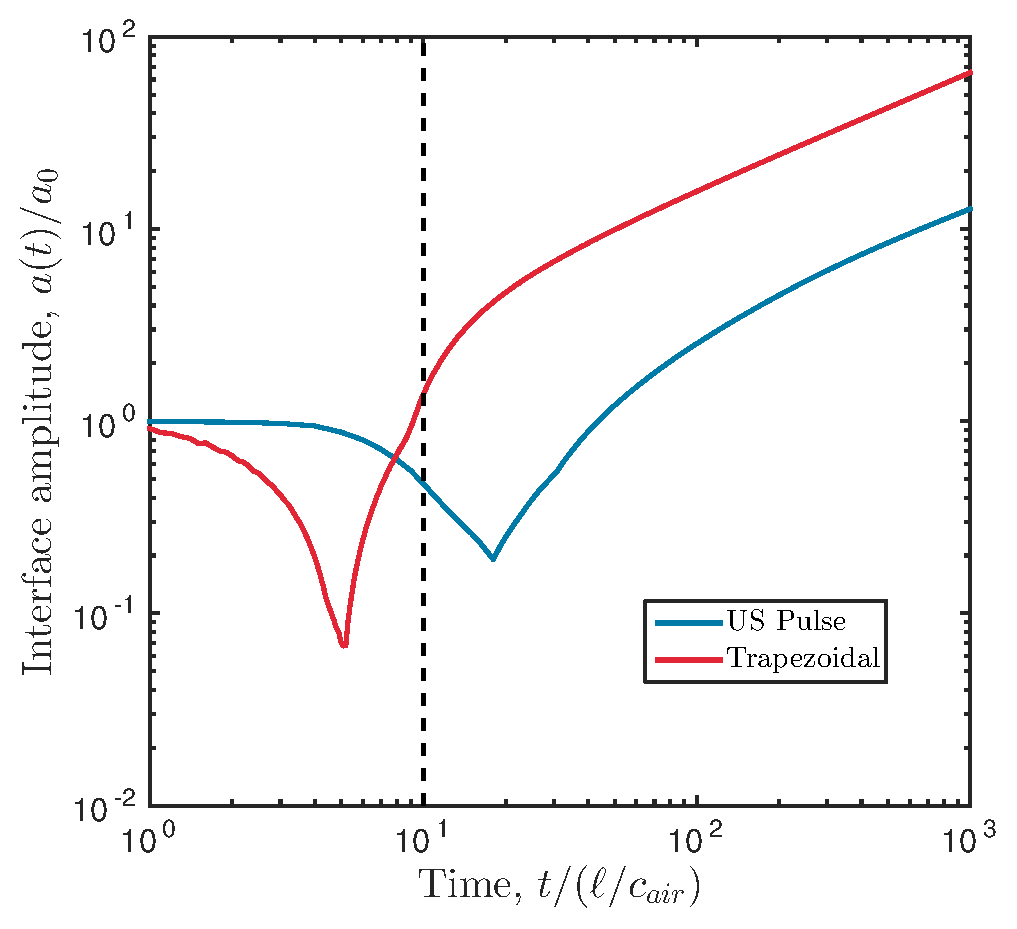
\includegraphics[width=\textwidth]{./figs/trapz_us_amp_comparison_A10_waveend}
    };%
    % \begin{scope}[x={(image.south east)},y={(image.north west)}]%
    %   \node[font=\scriptsize,align=left,right] at
    %   (0.2,0.9){{$t=1$}};%
    % \end{scope}%
  \end{tikzpicture}
  \caption[Interface perturbation amplitude history for the
  $p_a=10$ MPa ultrasound pulse.]{Interface perturbation amplitude
    history for the $p_a=10$ MPa ultrasound pulse. $a(t)/a_0$ is
    plotted vs time on a log-log scale. $t^{3/5}$ growth is
    indicated by the dashed black line.}
  \label{fig:us10_interface_growth}
\end{figure}%
% 
% In Chapter \ref{ch:usbe_lung} it was demonstrated that interface
% deformations that occurred following trapezoidal acoustic waves were
% indeed driven by baroclinic vorticity. And at the beginning of this
% chapter, we hypothesized that ultrasound waves may also be capable of
% generating baroclinic vorticity at alveolar interfaces within the
% lungs, and thus capable of inducing strains which may partially
% account for some of the lung hemorrhage observed as a result of
% \ac{DUS}. Unlike the trapezoidal waves of Chapter \ref{ch:usbe_lung},
% which had positive definite pressure profiles, the \ac{US} waves have
% cyclically positive and negative pressure profiles, which we
% intuitively expect to deposit vorticity of opposite sign on each
% subsequent cycle, and thus less total circulation after the passage of
% the wave.

After the passage of the \ac{US} pulse, there are no obvious
mechanisms, beside baroclinic vorticity, to drive the continued
deformation of the interface. As such, it is worth discussing what
precisely contributes to the circulation remaining after the passage
of the wave. Throughout the wave-interface interaction, the interface
itself deforms such that while \ac{US} pressure gradient is
continuously misaligned with portions of the interface density
gradient, though the degree of that misalignment changes in time along
the entire interface. While this deformation appears to be nominally
small (note the barely observable difference between frames 1 and 2
for each subfigure within Figures \ref{fig:rho_snapshots_A10},
\ref{fig:rho_snapshots_A25}, \ref{fig:rho_snapshots_A50}), it is
finite, calculable, and critical to the vorticity dynamics. Because
the pressure returns to ambient after the passage of the wave, it must
be true that the integral of the acoustic pressure gradient over all
time is zero, just as it was for the trapezoidal wave. Thus the only
way that baroclinic vorticity can remain after the passage of the wave
is through changes in the density gradient during the interaction. As the interface deforms
the direction these small changes in the direction and local magnitude
of the density gradient result in a net deposition of circulation that
remains to deform the interface after the passage of the wave. This
has particular relevance to ultrasound which relies on many subsequent
pulses, potentially resulting in the accumulation of vorticity over
time.
% 

\subsection{Limitations of the present work}
The model of an ultrasound-driven alveolus used in this work is
exactly that, a model. This work aims only to offer insight into the
physics and potential physical damage mechanisms of \ac{DUS}-induced
lung hemorrhage. Our approximation of the physical system is perhaps
not a particularly, naturally intuitive one. Moreover the vorticity
mechanisms that we suggest are driving the system are not intuitive
for a viscoelastic solid. The concept of vorticity, even in a
viscoelastic solid (e.g., soft tissue), can be thought of rather
simply at a fixed instant in terms of a velocity magnitude (not
direction) difference between opposite sides of a particle of
continuum, such that the instantaneous tendency of the particle is to
rotate. Our conceptual arguments for overcoming this arise out of our
understanding of this as a continuum of viscoelastic solids, which may
act as a solid or liquid depending on the physical regime of
interest. The model is based on highly fundamental laws of mechanics
(conservation of mass, momentum, energy) and neglected physical
effects are justified in the relevant regime based on dimensional
analysis. Additionally, the problem geometry and setup are chosen
based on the relevant application. While the author recognizes that
treatment of an alveolar septum as a perturbed water-air interface
intuitively seems a bit too simple, all of the dimensional and order
of magnitude arguments suggest that specifically for the timescales
considered here, the simulated dynamics are reasonable. Though there
are several limitations to this study that would not allow the
simulated physics to capture the physics of diagnostic
ultrasound-alveolar interactions over longer time spans. Here we
specifically consider limitations that arise from our constitutive
model of the lung tissue and the model problem geometry. Based on our
physical understanding, it is not unreasonable to speculate about how
each of these limitations is likely to effect the simulated physics.

In this study, we treat the alveolar septa and capillaries therein as
a liquid-gas interface, and within our physical model we neglect
certain physical features characteristic of soft tissue, including
viscoelasticity and the mechanical failure. Rather than repeat the
dimensional analysis arguments used to initially justify the model in
Chapters \ref{ch:Introduction} and \ref{ch:usbe_lung} we will consider
how each of these could affect the physical system. Viscosity and
elasticity both have potential importance at late times. In the
context of the present work, viscosity may act to serve as a mechanism
to dissipate vorticity, thus reducing strain on the
interface. However, the characteristic timescale over which we expect
the vorticity to dissipate over a relevant area $\sim\ell^2/\nu_{air}$
is multiple milliseconds, and is thus unlikely to greatly effect the
dynamics over the considered period. Elasticity is likely to provide a
restoring force to resist the deformation of the interface, however
this is likely to be small relative to the fluid inertia, which we
show quantitatively in Appendix
\ref{sec:elasticity_appendix}. Additionally, this model is no longer
valid after the alveolar septum fails, which may occur in some of our
simulations based on the considered failure criteria. As the strains
observed are large, before the elastic force is likely to overcome the
fluid inertia, the elastic restorative force may not be particularly
useful at mitigating vorticity-induced strain. Many of these specific
limitations are in part a result of limitations of the existing body
of knowledge concerning the mechanical properties and failure behavior
of alveolar tissue under stresses and strains, which is poorly
characterized within the timescales and physical regimes relevant
here. We highlight the fact that the available stress and strain
failure criteria available for alveoli are based on much slower
processes than occur during \ac{DUS}, making for an imperfect
comparison at best. Additionally, the stress $8$ kPa stress failure
criterion of \cite{West1991} is for wall stress, which is not the same
as shear, but was the best available metric at the time of this
writing.

In consideration of the limitations of our model geometry, we will
start from the fact that this work aims only to study interactions
between a single ultrasound pulse and a single alveolus. As such we
consider the effect of a treating the alveolar septum as a slightly
perturbed sinusoidal interface between fluids. In comparison to the
histological slide of alveoli shown in Figure
\ref{fig:alveolar_histology}, the geometry considered here is smoother
and flatter than true alveolar boundaries. As such, there is the
potential for greater shear stress concentrations and baroclinic
vorticity generation with subsequent strain in the real physical
system. Additionally, the 2D representation of the problem as a single
alveolus neglects any physical support the system may receive from its
surroundings. And while it has been suggested that pulmonary
capillaries are largely unsupported by surrounding tissues
\citep{West1991}, without quantification of that support, it is
possible that it would help to reduce vorticity-driven motion of the
interface, particularly at the edges. However, the deformation and
strain observed here is largely driven by vorticity local to the
interface perturbation, such that it would likely not be greatly
effected by such support. Lastly, we acknowledge that this model
cannot capture 3D fluid effects (e.g., turbulence, vortex-stretching,
etc...) that are expected to be negligible over the timescales
considered based on the Reynolds number and order of magnitude
analysis of the individual terms of the vorticity equation (see
Appendix \ref{sec:oom_analysis}).

\section{Summary, conclusions, and future work}
\label{sec:usbe_lung_bio_conclusions}
In summary, \ac{US} pulse waves were simulated propagating from water
into sinusoidally perturbed water-air interfaces to model a single
\ac{US}-pulse impinging upon an alveolus from surrounding soft
tissue. We assume a typical adult mean alveolar diameter of
$\ell=200~\mu$m \citep{Ochs2004} as a characteristic length scale,
such that the maximum simulation time was approximately $288~\mu$s. To
estimate viscous stresses and interfacial linear strains relevant to
\ac{DUS}-induced alveolar hemorrhage, 1.5 MHz ultrasound pulse waves
with amplitudes of $p_a=1.0, 2.5,$ and $5.0$ MPa were used. Initial
interface perturbation amplitudes of $a_0= 0.03\ell, 0.10\ell,$ and
$0.30\ell$ were considered. For each case, the wave-interface
interaction generated vorticity along the interface and resulted in
long-term deformation of the interface, which continued well after the
passage of the wave. Relevant calculations of the density fields,
inferred viscous stress fields, and linear interfacial strain within
the simulated period are reported. The computed peak interface strain
amplitudes $\abs{\varepsilon}$ ranged from $0.01$ to $0.38$. During
the computed period, only for the $5.0$ MPa wave did strains exceed the
$\abs{\varepsilon}=0.08$ damage threshold, reported by
\cite{Belete2010}. The peak passive viscous stress estimates at the
interface were on the order of tens of Pascals, which is far below the
$8$ kPa stress failure criterion reported by \cite{West1991}. A second
experiment was performed to determine that baroclinic vorticity is the
driver of the observed deformation. For this experiment, a $p_a = 10$
MPa pulse was propagated toward a perturbed water-air interface of
amplitude $a_0 = 0.03\ell$ and the vorticity and interface dynamics
were compared to those of the trapezoidal waves in Chapter
\ref{ch:usbe_lung}. It was found that ultrasound pulses deposited
circulation of similar distribution and order of magnitude to those
previously observed for the trapezoidal waves. The perturbation was found
to grow approximately as $t^{3/5}$, as was expected for baroclinic
vorticity-driven growth, based on our previous work.

This work is a first step toward investigating the possibility of
baroclinic vorticity-induced strain as potential mechanism for
ultrasound-induced alveolar hemorrhage. This work is novel in its
modeling using the nonlinear equations of fluid motion to study the
dynamics of an alveolus interacting with a single \ac{DUS}
pulse. Furthermore, this work is unique in its comparison of alveolar
stress and strain estimates with previously determined failure
criteria. While the calculated stresses and strains observed based on
the interaction between an air water interface and a single ultrasound
pulse may be representative of some of the physics associated with
\ac{DUS}-alveolar interactions, we cannot confidently say that
baroclinic vorticity is the likely cause of \ac{DUS}-induced
hemorrhage in the lung. As true \ac{DUS} typically involves many
subsequent pulses, further investigations will need to account for
this. However, based on the work reported here, we draw the following
conclusions:
\begin{enumerate}
\item \textbf{Newtonian, viscous stress alone is unlikely to be
    sufficient to cause \ac{DUS}-induced hemorrhage of the alveolar
    wall}. While many approximations and simplifications were made
  throughout the course of this work, the work presented estimates
  \textit{worst case} viscous shear stresses. Here, the velocity
  gradients are higher than would be expected in the true physical
  system because neglected viscous and elastic effects would resist
  interfacial motion in the true physical system. In spite of this,
  the calculated shear stresses are multiple orders of magnitude less
  than expected alveolar stress failure thresholds.
\item \textbf{\ac{DUS} pulses within clinically relevant regimes have
    the potential to deposit baroclinic vorticity within gas-liquid
    interfaces in the lungs, which is capable of driving deformation.}
  This work clearly demonstrates that diagnostically relevant
  ultrasound pulses are capable of creating lasting baroclinic
  vorticity at liquid-gas interfaces which are dynamically similar to
  alveolar tissue-gas interfaces. For the $10$ MPa case, the interface
  perturbation exhibits $\sim t^{3/5}$ power-law growth at late times,
  as was previously shown to occur for interfaces driven by
  trapezoidal acoustic waves. For weaker waves, running the
  simulations to sufficiently late time to observe this behavior was
  too computationally costly to be done. This indicates that
  ultrasonically driven vorticity is a viable mechanism for driving
  the observed growth. The observed interfacial strains created by
  pulses as weak $p_a = 5.0$ MPa were more than sufficient to cause
  damage based on previously observed alveolar failure
  criteria. Furthermore, based on dimensional arguments, dissipation
  of the observed vorticity is expected to occur over multiple
  milliseconds, which is greater than the typical time between
  subsequent \ac{DUS} pulses. Hence \ac{US} may be capable of
  accumulating vorticity in the lungs over several subsequent pulses
  and thus driving greater deformation. This will depend on the
  morphology of the interface during the arrival of each pulse, which
  is likely to vary widely depending on the initial conditions and
  ultrasound parameters, as the minimum strain cases showed
  practically no deformation over a third of a typical pulse interval,
  and the large strain cases are likely to cause alveolar failure
  before subsequent pulses arrive. 
\end{enumerate}



%%%%%%%%%%%%%%%%%%%%%%%%%%%%%%% 
% \section{conclusions and future work}


% \begin{comment}
%   Among the tissue layers%   The anatomical structure of the lungs has been studied extensively
%   and is of particular interest to the present work. The alveoli can
%   be thought of as a network of openly connected, air-filled saccules
%   with distinctly irregular surfaces. And while alveoli are
%   irregularly shaped and do not have a true diameter, past research
%   suggests that their size appear to be species dependent
%   \citep{Faffe2002}. Mean valveolar diameters range from tens to
%   hundreds of microns with reported values of 45 $\mu$m in mice
%   \cite{Knust2008} and 200 $\mu$m in adult humans \cite{Ochs2004} for
%   examples. The septa that separate adjacent alveoli are nearly planar
%   structures that contain several tissue layers and are coated with a
%   thin layer of liquid surfactant
%   \citep{Gil1979,Reifenrath1975,Perlman2014}.
%   The extreme thinness of this barrier is necessary
%   for efficient gas exchange. The physical dimensions of the alveolus
%   and thinness of this barrier relative to typical \ac{US} wavelengths
%   are of importance to the model used in this study.

%   In addition to anatomical structure, the mechanical properties and
%   failure behavior of alveoli and other relevant pulmonary tissues
%   have been studied extensively in computational and animal
%   models. \cite{Perlman2014} combined experimentally measured strains
%   with computationally modeled lung stresses to demonstrate that the
%   effective Young's moduli of aveolar septa depend on transpulmonary
%   pressure. Values range from a minimum of $E_a=12$ kPa in the low
%   transpulmonary pressure range of $\approx 0.4$-$0.6$ kPa to a
%   maximum $E_a=140$ kPa at a high transpulmonary pressure of range,
%   $\approx 1.5$-$2.5$ kPa. \cite{West1991} raised the pulmonary
%   capillary pressure of anesthetized rabbits and observed consistent
%   stress failure of the capillary and alveolar epithelium for
%   transmural at or above $40$ mmHg ($5.3$ kPa). It was observed that
%   failure corresponded to approximately $25$ mN/m wall tension in the
%   capillaries, and noted that ``this tension is small, comparable with
%   the tension in the alveolar wall associated with elastic recoil.''
%   The capillary wall stress at failure was calculated to be
%   approximately $8$ kPa.%

%   %   \begin{comment} This is roughly consistent with \cite{Welling1972}
%   %     which measured properties of basement membranes from rabbit renal
%   %     tubules and showed that a $57 \mu$m tubule could withstand $4.1$
%   %     kPa transmural pressure, which, based on a Laplace relationship,
%   %     equates to an ultimate tensile strength of 500 kPa
%   %     \citep{West1999}. Furthermore, \cite{Welling1972} also showed that
%   %     properties of these tubules depended only on the strength of their
%   %     basement membrane.
%   %   \end{comment}%

%   Alveolar strain response has also been previously studied. Linear,
%   alveolar strain due to normal tidal breathing is in the range of
%   $0$-$5$\% for humans \citep{Roan2011}. And \cite{Vlahakis2000} reports that
%   alveolar plasma membranes resist lateral tension and fail under
%   stresses greater than $0.4-0.6$ Pa, which corresponds to strains of
%   $2-3\%$. However, this work also acknowledges that typical changes in
%   cellular surface area are primarily a result of plasma membrane
%   unfolding and not actual wall strain. \cite{Belete2010} found that
%   when subjected to cyclical linear stretch at 0.5 Hz for 30 minutes,
%   rat alveolar epithelial cells experiencing Linear strains of $8\%$ or
%   greater were frequently damaged, whereas those experiencing strains
%   of $3 - 6\%$ often undamaged. 


%   \hl{ELASTICITY STUFF}
%   \cite{Perlman2014}
%   combined experimentally measured strains with computationally modeled
%   lung stresses to demonstrate that the effective Young's moduli of
%   aveolar septa depend on transpulmonary pressure. Values range from a
%   minimum of $E_a=12$ kPa in the low transpulmonary pressure range of
%   $\approx 0.4$-$0.6$ kPa to a maximum $E_a=140$ kPa at a high
%   transpulmonary pressure of range, $\approx 1.5$-$2.5$
%   kPa.

% \end{comment}










% \begin{comment}
%   %   \section{Results and discussion}
%   %   \subsection{Stresses and strains in the lungs}
%   %   Lung tissue has been recognized to exhibit viscoelastic behavior
%   %   since as early as 1939 \citep{Bayliss1939}. As a result of this,
%   %   we consider both viscous and elastic stress as potential damage
%   %   mechanisms underlying ultrasound-induced lung hemorrhage.

%   %   \subsubsection{Viscous Stresses}
%   %   \begin{figure}
%   %     \centering
%   %     
\includegraphics{./figs/placeholder}
%   %     \caption{Plot of maximum viscous stress vs time for US pulse
%   %     waveforms.}
%   %   \end{figure}

%   %   \subsubsection{Elastic Stresses}
%   %   \begin{figure}
%   %     \centering
%   %     
\includegraphics{./figs/placeholder}
%   %   %     \caption{Plot of engineering strain vs time. Strain on left
%   %   %     side, stress on right side, dashed line at 500 kPa, which is
%   %   %     failure based on \cite{West1999}.}
%   %   \end{figure}
% \end{comment}


% \begin{comment} %This is pretty much all in the previous chapter
%   The physical mechanisms underlying \ac{DUS}-induced \ac{PH} are not
%   well understood and traditionally expected \ac{US} bioeffects
%   mechanisms do not appear to be the primary cause of damage. \ac{US}
%   bioeffects mechanisms are typically classified as thermal or
%   non-thermal with the bulk of non-thermal bioeffects being a result
%   of acoustic \ac{IC}. \cite{Zachary2006} finds that \ac{DUS}-induced
%   lung lesions do not appear similar to those induced by heat and
%   concludes that thermal mechanisms are not likely to be the
%   cause. \cite{OBrien2000} observes that the severity of
%   \ac{DUS}-induced \ac{LH} in mice increases under raised hydrostatic
%   pressure, and \cite{Raeman1996} finds that the \ac{LH} is unaffected
%   by the introduction of \ac{US} contrast agents. Both of these
%   findings are inconsistent with what would be expected of
%   \ac{IC}-induced hemorrhage. One study reports detecting cavitation
%   during \ac{DUS}-lung interaction in rats
%   \cite{Holland1996}. \cite{Tjan2007} considers another potential
%   damage mechanism, that focused \ac{US} may lead to the ejection of
%   droplets capable of puncturing the air-filled sacs within the
%   lung. To investigate this, they perform numerical simulations of as
%   an inviscid, free surface subjected to a Gaussian velocity potential
%   and show show that the proposed droplet ejection may occur under
%   certain circumstances. Similarly, \cite{Simon2012} observed
%   \ac{HIFU} induced atomization of tissue at air interfaces. Despite
%   these efforts, the precise damage mechanism underlying
%   \ac{DUS}-induced \ac{LH} is still unknown.
% \end{comment}

% % This is probably all in the last chapter or the introduction. Just add a paragraph relating the last chapter to this one here
% \begin{comment}
%   Previously there has been extensive research
%   investigating interactions between fluid-fluid interfaces driven by
%   mechanical waves. Much of this work has been motivated by man-made
%   applications such as inertial confinement fusion and astrophysical
%   phenomena such as supernova collapse. Accordingly much of the previous
%   research has focused on shock-accelerated, perturbed interfaces
%   between fluids of different densities
%   \citep{Brouillette2002}. \cite{Taylor1950} performed linear stability
%   analysis for the case of a perturbed interface between two fluids
%   undergoing constant acceleration, e.g., gravity. Taylor found that
%   under certain configurations the interface perturbation
%   grows. \cite{Richtmyer1960} extended this linear analysis to the case
%   of an impulsively accelerated interface to create a model for the
%   initial growth of a shock-driven interface perturbation. Later,
%   \cite{Meshkov1969} experimentally confirmed Ricthmyer's qualitative
%   predictions. Hence the growth of a shock-driven fluid-fluid interface
%   has been labeled as the \ac{RMI}. To lend physical insight into the
%   underlying mechanism behind this, \cite{Hawley1989} demonstrated that
%   this phenomenon could be described using vortex deposition-evolution
%   paradigm. The basic mechanism driving the growth of the perturbation
%   in the case of the \ac{RMI} is baroclinic vorticity created by the
%   misalignment of the pressure gradient across the shock and the density
%   gradient at the interface. Recently \hl{Patterson \& Johnson
%   (submitted, 2016)} performed numerical experiments and analysis to
%   show that for the case of liquid-gas interfaces, acoustic waves may
%   also be capable of depositing sufficient baroclinic vorticity at the
%   interface to cause significant deformation, as a result of the sharp
%   density gradient across the interface.
% \end{comment}


% \begin{comment}
%   %   \subsection{Summary}
%   As \ac{DUS} of the lung has been shown to trigger same-day, acute
%   alveolar hemorrhage \cite{Zachary2001}, it is specifically
%   interactions between the an aveolus and a single \ac{DUS} pulse that
%   we consider in this work. To investigate the mechanism underlying this
%   hemorrhage, we develop a numerical model of this problem to compute
%   the expected dynamics of the alveolar air-tissue interface for varying
%   acoustic amplitudes an alveolar geometries. To relate the computed
%   dynamics to lung hemorrhage, we approximate the relevant stresses and
%   strains and compare these results to existing values of the material
%   properties alveolar tissue to assess possible causes of hemorrhage.

%   \hl{OUT OF PLACE:\\
%   This work aims to use numerical simulations to investigate the
%   dynamics associated with the interaction between an ultrasound pulse and
%   an aleolar air-tissue interface. We hypothesize that acoustically
%   generated baroclinic vorticity within the lungs is capable of driving
%   deformation of alveolar air-tissue interfaces to the point of
%   hemorrhage. We model the problem as a sinusoidally perturbed air-water
%   interface driven by a single acoustic pulse and study the subsequent
%   dynamics. Calculated stresses and strains are compared to previously
%   measured failure criteria from the literature.}

% \end{comment}

% % This is the old methods section, that now largely exists in the previous chapter.
% \begin{comment}
%   \section{Methods}
%   In this section we develop a model of \ac{DUS}-alveolus interaction
%   as a compressible fluid system. We then describe in detail the setup
%   of the numerical experiments performed and calculations performed to
%   investigate the problem. 

%   \subsection{A model of \ac{DUS}-alveolus interaction}
%   \hl{COPIED THIS PARAGRAPH TO OTHER PAPER}.  Consider a \ac{DUS} pulse
%   as it travels into the lungs. After passing through layers of soft
%   tissue and fluid, the wave encounters a network of openly connected,
%   air-filled saccules with distinctly irregular surfaces. These are the
%   alveoli. It is the interaction between an incident \ac{US} pulse and
%   the first alveolar tissue-air interface it encounters that we treat
%   here, as shown in figure \ref{fig:alveolar_schematic}.

%   To model the problem, we consider a rectangular domain with a 2D
%   $(x,y)$ cross section containing soft tissue (modeled as water)
%   sitting atop a single alveolus (modeled as air) as illustrated in
%   figure \ref{fig:ic_schematic}. An acoustic pulse is prescribed within
%   the water, above the interface, and allowed to propagate downward
%   ($-y$-direction) toward the air. The alveolus spans the width of the
%   domain, $\ell$. A typical mean aveolar diameters in an adult human is
%   $200 \mu$m \citep{Ochs2004}.

%   To capture the irregular shape of the alveolus, the water-air
%   interface contains a single mode sinusoidal perturbation of amplitude
%   $a_0$ such that the vertical center of the interface is described by,
%   \begin{align} %Not y_interface in the code
%     Y(x,t=0)_{interface} = a_0\sin\left(\frac{2\pi x}{\ell}-\frac{\pi}{2}\right). 
%   \end{align}
%   An interface thickness $\delta=0.08$ is chosen such that at $t=0$, the
%   fluid in the domain above $y\geq Y_{interface}+\delta/2$ is pure
%   water, and below $y\leq Y_{interface}-\delta/2$ is pure air, which a
%   water-air mixture filling the region around the interface. A more
%   detailed treatment of the interface can be found in referred to
%   \hl{(Patterson and Johnsen, 2016)}. To investigate the dependence of
%   the dynamics on the alveolar geometry we will consider multiple
%   interface perturbation amplitudes: $a_0=0.03\ell, 0.10\ell, 0.2\ell,$
%   and $0.30\ell$.

%   The diagnostic ultrasound pulse is modeled as a sinusoidal carrier
%   wave of amplitude $p_a$ and frequency $f$ modulated by a Gaussian
%   Envelope such that,
%   \begin{align}
%     p(x,t_0) = p_a\sin{\left(2\pi f\frac{\left[y-\left(Y_{wave}+L_{wave}\right)\right]}{c}\right)}\exp{\left(-\frac{\left(\left[y-\left(Y_{wave}+L_{wave}/2\right)\right]c\right)^2}{FWHM/\left(2\sqrt{2\ln{\left(2\right)}} \right)}\right)}.%
%   \end{align}
%   The carrier wavelength $\lambda=c_{water}/f$ and the full width of the
%   Gaussian envelope at half of the maximum amplitude $FWHM$ are designed
%   to scale appropriately with respect to $\ell$. Here,
%   $f\approx 1.25 c_{water} / 2\pi \ell$ and $FWHM=15\ell$. For an
%   alveolar length scale of $\ell=200 \mu$m, this corresponds to $f=1.65$
%   MHz and $FWHM=3$ mm. $L_{wave}=45\ell$ is the length of the
%   computational domain, over which the wave is defined to exist and
%   $Y_{wave}$ is $y$-location of the bottom of the wave at $t=0$, which
%   is set to $10a_0$ above the peak of the interface. To consider the
%   dependence of the interface dynamics on pulse amplitude we vary
%   $p_a = 1, 5, 10,$ and $15$ MPa.

%   \subsection{Governing Equations}
%   To simulate the model problem described above we solve equations for
%   conservation of mass, momentum, energy. While it has been long since
%   recognized that tissue exhibits viscoelastic behavior
%   \citep{Bayliss1939}. To simplify things we consider the expected
%   length scale over which viscosity will influence the dynamics,
%   $l_{viscous}$. From dimensional analysis, this scales as
%   $l_{viscous}\sim\sqrt{\nu/(\ell/c)}$. In air at 300 K,
%   $l_{viscous}\sim\orderof{1 \mu\text{m}}$ and in water
%   $l_{viscous}\sim\orderof{0.1 \mu\text{m}}$. In either case we consider
%   that $l_{viscous}<<\ell$. \hl{Furthermore, we consider the relative
%   importance of elasticity and surface tension }

%   \begin{comment}
%     \begin{itemize}
%     \item $c_{air} = 347.2$ m/s
%     \item $c_{water} = 1500$ m/s
%     \item $\nu_{air} = 1.568\times 10^{-5}$ m$^2$/s
%     \item $\nu_{water} = 0.8539\times 10^{-6}$ m$^2$/s
%     \item $G_{alveolar-wall} = 5$ kPa \cite{Cavalcante2005}
%     \item $\sigma_{water}=0.072$ at N/m 298K
%     \item $\rho_{air}=1.1765$ kg/m$^3$
%     \item $\rho_{water}=996$ kg/m$^3$
%     \item if $p_a=1 MPa$:
%       \begin{itemize}
%       \item $u_{acoustic-water}\approx0.6$ m/s
%       \item $u_{acoustic-air}\approx1.2$ m/s
%       \end{itemize}
%     \item $Re=\frac{\rho u}{\nu}$ =
%     \item $We=\frac{\rho u^2 \ell}{\sigma}$ = $(\infty)_{air}$ =
%       $()_{water}$
%     \item $Ca=\frac{\rho u^2}{K}$
%     \end{itemize}
%   \end{comment}

%   \begin{subequations} \label{eq:euler}%
%     \begin{align}%
%       \frac{\partial \rho}{\partial t} + \frac{\partial \left(\rho u\right)}{\partial x} + \frac{\partial \left(\rho v\right)}{\partial y} = 0,\\
%       \frac{\partial \rho u}{\partial t} + \frac{\partial}{\partial x}\left( \rho u^2+p\right)  + \frac{\partial}{\partial y}\left( \rho uv\right) = 0,\\
%       \frac{\partial \rho v}{\partial t} + \frac{\partial}{\partial x}\left( \rho uv\right)  + \frac{\partial}{\partial y}\left( \rho v^2+p\right) = 0,\\
%       \frac{\partial E}{\partial t} + \frac{\partial}{\partial x}\left[u\left(E+p\right)\right] + \frac{\partial}{\partial y}\left[v\left(E+p\right)\right] = 0,
%     \end{align}%
%   \end{subequations}%


%   \subsection{Computational implementation}
%   The Euler equations \eqref{eq:euler} are solved on a rectangular
%   computational grid using Discontinuous Galerkin Methods in space and a
%   fourth order Runge-Kutta time marching scheme as described in
%   (Patterson and Johnsen, 2016 [submitted]). As previously mentioned the
%   width of the computational domain is 1 mean alveolar diameter,
%   $\ell$. The length of the domain is chosen based on two criteria: one
%   - the domain must fully capture the initial acoustic wave and the
%   moving interface throughout the simulation, and two - the domain must
%   be long enough to sufficiently largely eliminate artificial
%   reflections from the boundaries. Thus the computational domain
%   considered for this problem is described by $0\leq x\leq1\ell$ and
%   $-20\ell\leq y\leq 60\ell$. To further help eliminate reflections,
%   grid stretching is implemented at the top and bottom $10\ell$.

%   - Wave
%   \begin{itemize}
%   \item ultrasound is focused to a zone that is at least of order
%     $\lambda$, and $\lambda>>\ell.$
%   \item $k_{y-acoustic}/1.25$
%   \end{itemize}


%   -length scales
% \end{comment}
% 
%%%%%%%%%%%%%%%%%%%%%%%%%%%%%%%%%%%%%%%%%%%%%%%%%%%%%%%%%%%%% 
% VORTICITY SNAPSHOTS %%%%%%%%%%%%%%%%%%%%%%%%%%%%%%%%%%%%%%%
%%%%%%%%%%%%%%%%%%%%%%%%%%%%%%%%%%%%%%%%%%%%%%%%%%%%%%%%%%%%% 
% Figure \ref{fig:us_vorticity_snapshots} illustrates the vorticity
% field at $t=1, 10, 100, and 500$ for $p_a = 2.5$
% \ref{fig:vorticity_snapshot_A25_a03} and $5$ MPa
% \ref{fig:vorticity_snapshot_A50_a03} for $a_0 = 0.03\ell$. The $1$ MPa
% case is excluded because little deformation was observed over the
% simulated period. $a_0 = 0.03\ell$ is chosen, as this is the case in
% which the least baroclinic vorticity expected because of greater
% alignment between the ultrasound pressure and interface density
% gradients. 
% % 
% \hl{BETTER SNAPSHOTS}
% \begin{figure}
%   \centering
%   \begin{subfigure}[b]{0.9\textwidth}
%     \begin{tikzpicture}%
%       \node[anchor=south west,inner sep=0] (image) at (0,0) {
%       \includegraphics[width=\textwidth]{./figs/lung_figs/rmawave_1_A25_a03_t500_vorticity_snapshots}
%     };%
%       \begin{scope}[x={(image.south east)},y={(image.north west)}]%
%         \node[font=\normalsize,right] at (0.07,0.13) {$t=1$};%
%         \node[font=\normalsize,right] at (0.28,0.13) {$t=10$};%
%         \node[font=\normalsize,right] at (0.5,0.13) {$t=100$};%
%         \node[font=\normalsize,right] at (0.73,0.13) {$t=500$};%
%       \end{scope}%  
%     \end{tikzpicture}%
%     \caption{\label{fig:vorticity_snapshot_A25_a03} $p_a = 2.5$ MPa, $a_0 = 0.03\ell$}
%   \end{subfigure}
%   %   
%   \begin{subfigure}[b]{0.9\textwidth}
%     \begin{tikzpicture}%
%       \node[anchor=south west,inner sep=0] (image) at (0,0) {
%       \includegraphics[width=\textwidth]{./figs/lung_figs/rmawave_1_A50_a30_t500_vorticity_snapshots}
%     };%
%       \begin{scope}[x={(image.south east)},y={(image.north west)}]%
%         \node[font=\normalsize,right] at (0.07,0.13) {$t=1$};%
%         \node[font=\normalsize,right] at (0.28,0.13) {$t=10$};%
%         \node[font=\normalsize,right] at (0.5,0.13) {$t=100$};%
%         \node[font=\normalsize,right] at (0.73,0.13) {$t=500$};%
%       \end{scope}%  
%     \end{tikzpicture}%
%     \caption{\label{fig:vorticity_snapshot_A50_a30} $p_a = 5$ MPa, $a_0 = 0.30\ell$}
%   \end{subfigure}
%   \caption{Snapshots of the vorticity field at $t=1, 10, 100,$ and
%   $500$ are shown for two example cases. Figure
%   \subref{fig:vorticity_snapshot_A25_a03} shows the vorticity
%   fields for the case for which very little late time deformation
%   occurs, in which $p_a = 2.5$ MPa, $a_0 = 0.03\ell$. Figure
%   \subref{fig:vorticity_snapshot_A50_a30} shows the vorticity
%   fields for the case for which there is significant late late-time
%   deformation of the interface, in which $p_a = 5$ MPa,
%   $a_0 = 0.30\ell$.}
%   \label{fig:us_vorticity_snapshots}
% \end{figure}
% 

% \begin{comment}
%   \begin{align}
      %       p(y,t_0) = p_a\sin{\left(2\pi f\frac{\left[y-\left(Y_{wave}+L_{wave}\right)\right]}{c}\right)}\exp{\left(-\frac{\left(\left[y-\left(Y_{wave}+L_{wave}/2\right)\right]c\right)^2}{FWHM/\left(2\sqrt{2\ln{\left(2\right)}} \right)}\right)}.%
      %     \end{align}
      % %     
      %       The carrier wavelength $\lambda=c_{water}/f$ and the full width of
      %       the Gaussian envelope at half of the maximum amplitude, or $FWHM$,
      %       are designed to scale appropriately with respect to $\ell$. Here, we
      %       choose design parameters of $f\approx 1.25 c_{water} / 2\pi \ell$
      %       and $FWHM=15\ell$ such that for an alveolar length scale of
      %       $\ell=200 \mu$m, the corresponding center frequency is $f=1.65$ MHz
      %       and $FWHM=3$ mm. $L_{wave}=45\ell$ is the length of the portion of
      %       the computational domain, over which the wave is defined to exist,
      %       such that the approximate duration of the wave-interface interaction
      %       is just under $6 \mu$s. $Y_{wave}$ is the $y$-location of the bottom
      %       of the wave at $t=0$, which is set to $10a_0$ above the peak of the
      %       interface.
      %       \end{comment}
      %       \begin{comment}
      %       \begin{align}
      %       \label{eq:p0}
      %       p(y_f,t=0) = p_{atm} + p_a %
      %       \begin{cases}
      %       0,&y_f\leq0 ,\quad$or$\quad y_f\geq45\ell,\\%
      %       \frac{y_f}{5\ell},&0\leq y_f\leq5\ell,\\%
      %       1,&5\ell\leq y_f\leq40\ell,\\%
      %       1-\frac{y_f-40\ell}{5\ell},\qquad\qquad\qquad&40\ell\leq y_f\leq45\ell,%
                                                             %                                                              \end{cases}%
                                                             %     \end{align}
                                                             %                                                              where $y_f = y - (a_0+0.30\ell)$ is the $y$-location, relative to the
                                                             %                                                              initial location of the wave leading end. At these amplitudes and
                                                             %                                                              frequencies, linear acoustics describes ultrasound propagation in
                                                             %                                                              homogeneous tissue, such that the initial $x-$ and
                                                             %                                                              $y-$velocity components are set to $u=0$ and
                                                             %                                                              $v=-\Delta p_a / (\rho c)$, respectively, and initial density is
                                                             %                                                              $\rho_{water} + \Delta p_a / c^2$ \citep{Anderson1990}, where
                                                             %                                                              $\Delta p_a=p(y,0)-p_{atm}$ is the acoustic perturbation pressure.
                                                             %                                                              \end{comment}


%%% Local Variables:
%%% mode: latex
%%% TeX-master: "../../main"
%%% End:
